\documentclass[journal,twoside,web]{ieeecolor}
\usepackage{generic}
\usepackage{cite}
\usepackage{amsmath,amssymb,amsfonts}
\usepackage{algorithmic}
\usepackage{graphicx}
\usepackage{textcomp}
\usepackage{algorithm}
\usepackage{stfloats}
\usepackage{subfigure}
\usepackage{booktabs}
\usepackage{multirow}


\newtheorem{remark}{Remark}

\def\BibTeX{{\rm B\kern-.05em{\sc i\kern-.025em b}\kern-.08em
    T\kern-.1667em\lower.7ex\hbox{E}\kern-.125emX}}
\markboth{\journalname, VOL. XX, NO. XX, XXXX}
{Yu \MakeLowercase{\textit{et al.}}: A Hybrid Neurodynamic Scheme for Bimanual Synchronized Tracking Control of Robotic Manipulators}
\begin{document}
\title{A Hybrid Neurodynamic Scheme for Bimanual Synchronized Tracking Control of Robotic Manipulators with Uncertain Kinematics}
\author{Peng~Yu, Ning~Tan,~\IEEEmembership{Senior Member,~IEEE}, and Xiaoyi Gu
\thanks{This work was supported in part by the National Natural Science Foundation of China under Grant 62173352 and in part by the Guangdong Basic and Applied Basic Research Foundation under Grant 2024B1515020104. (\textit{Corresponding authors: Ning Tan, Xiaoyi Gu})}
\thanks{P. Yu and N. Tan are with the School of Computer Science and Engineering, Sun Yat-sen University, Guangzhou, China. (e-mail: tann5@mail.sysu.edu.cn)}
\thanks{X. Gu is with Joyo Medtech (Suzhou) Co., Ltd, Suzhou, China. (e-mail: 7520230183@bit.edu.cn)}}

\maketitle

\begin{abstract}
The reconfigurability and structural complexity of robotic manipulators introduce significant challenges to their kinematic modeling, making traditional model-based methods less feasible. This paper studies the synchronized tracking control problem of a dual-arm system with completely unknown kinematic model for the first time. A gradient neurodynamic method is presented to learn the unknown Jacobian matrices of dual manipulators. Then, we innovatively employ the coupled error in dual quaternion form as the state function of the zeroing neurodynamic model to control position and orientation simultaneously, leading to a more streamlined and compact inverse kinematics solution. Furthermore, by transforming task-space coupled errors into joint-space errors, we improve the cerebellar neural network to a mode compatible with kinematic control and, for the first time, utilize it to optimize synchronized kinematic control. Finally, the effectiveness of the proposed method is validated by simulations and experiments on various robotic manipulators. 
\end{abstract}

\begin{IEEEkeywords}
Bimanual operation, dual robotic manipulators, hybrid neurodynamics, uncertain kinematics.
\end{IEEEkeywords}

\section{Introduction}

Compared to a single robotic manipulator, dual robotic manipulators offer wider workspace, greater payload capacity for handling heavy objects~\cite{Caccavale2008}, and increased flexibility for managing complex tasks~\cite{Jin2023TII}. Consequently, the design of cooperative control methods for dual robotic manipulators has garnered significant attention in academia. This paper seeks to address the problem of bimanual synchronized kinematic control of dual robotic manipulators with uncertain kinematics.

Typically, the kinematic model of a robotic manipulator is parametrized using the Denavit-Hartenberg (DH) convention, which has led to the development of numerous control methods~\cite{Zhang2022}. However, as task complexity increases, robotic manipulators are becoming increasingly complex and reconfigurable, rendering these kinematic parameters unavailable in some cases. For example, a robotic manipulator equipped with a flexible end tool may deform unpredictably upon contact with the environment during the task~\cite{Wang2023}. In these scenarios, where prior knowledge of the robot kinematics is partially known or absent, model-based methods become infeasible. Therefore, designing control systems capable of learning uncertain robot model is essential~\cite{DallaLibera2021}.

Model-free kinematic control of robotic manipulators has been extensively studied over the past decades. A common approach is to estimate the unknown Jacobian matrix and design a controller at the velocity level~\cite{Liu2022b}. However, most existing methods require various feedback information, including the end-effector position, velocity and acceleration, some of which are difficult to measure in practice. Some methods directly learn the inverse kinematics of a robotic manipulator~\cite{Kim2021}, mapping task-space movement to joint angle command. However, these learning-based methods require massive data for offline training. Once the robotic manipulator or the end tool is changed, the offline training must be repeated to ensure accuracy, greatly increasing human burden and reducing the adaptability of these methods. Additionally, other prevalent model-free methods linearize the kinematic model as the product of a regression matrix and a parameter vector~\cite{Wang2017b}. However, as pointed out in the literature~\cite{Tarokh2021}, the calculation of the regression matrix is very complex for robotic manipulators with more than 2 or 3 degrees of freedom (DOF), limiting this approach to planar robots. Therefore, developing an efficient control system for high-DOF robotic manipulators with uncertain kinematics remains a significant research challenge.

Dual robotic manipulators are essential in scenarios where tasks are too complex for a single robotic manipulator~\cite{Yang2017,Zhang2023,Huang2023TII}. In the tracking control problem of dual robotic manipulators, one of the major challenges is to achieve pose synchronization between the manipulators. In several coordinated motion control methods for dual or multiple robots~\cite{Zheng2024TII,Jin2018,Chen2020}, controllers were designed separately for each manipulator without considering pose synchronization. In~\cite{Sun2002}, synchronization functions were defined to describe the kinematic relationship between different robots, which only considered the uncertain dynamics of robots, assuming the kinematics is available. Synchronized control of dual robotic manipulators with uncertain kinematics and dynamics has also been reported~\cite{Zhai2022}. However, this method requires the decomposition of robot kinematics and dynamics into a regression matrix and a parameter vector, which suffers from the aforementioned problem. Unlike existing methods, this paper seeks to develop a bimanual synchronized tracking control method for dual robotic manipulators that is suitable for high-DOF robotic manipulators (6-DOF or 7-DOF) and does not require analytical robot kinematics or offline training.


Humans demonstrate superb dual-arm control ability, coordination capability, and rapid learning ability, inspiring the integration of underlying biological mechanisms into control system design. Existing studies have shown that the cerebellum is prominent among central nervous system regions associated with motion control due to its crucial role in integrating, regulating and coordinating motion process and motion learning~\cite{Yan2023TCDS,Abadia2021,Tolu2020}. However, to the best of our knowledge, the cerebellum-inspired synchronized control of dual robotic manipulators is still unexplored. There are two main difficulties in applying cerebellum-inspired synchronized control to dual robotic manipulators. First, when applying a cerebellum model, dimensions of the actuation space and task space of robots should be consistent~\cite{Tolu2020,Capolei2020,Abadia2021}, which usually holds in joint-space dynamic control. However, this work focuses on the kinematic control of dual robotic manipulators, where the actuation space and the task space have different dimensions, making it difficult to directly apply cerebellum-inspired methods. Second, when controlling a single robotic manipulator, the cerebellum model only needs to compensate for the task-space tracking error. However, when controlling dual robotic manipulators, the cerebellum model needs to compensate for synchronization error, as well as task-space tracking error, making it difficult to choose appropriate input signal and teaching signal for the cerebellum model.

To sum up, this paper makes the following contributions:

\begin{enumerate}


\item This paper studies the synchronized tracking control problem of a dual-arm system with completely unknown kinematic models for the first time. By proposing a hybrid neurodynamic approach, we enable the online learning of robot models and synchronized control. Compared to existing model-based methods~\cite{Chen2020,Zhang2021TNNLS,Jia2020Robotica,Zhan2024TNNLS}, our method can avoid the complex analytical modeling procedure, allowing for rapid adaptation to different types of high-DOF robotic systems.

\item This is the first work that employs the coupled error in dual quaternion form as the state function of the zeroing neurodynamic model, enhancing its problem-solving capability. Unlike previous approaches that require two separate models to control position and orientation respectively~\cite{YANG2021108007,Li2024TII}, our method unifies both aspects within a single model, leading to a more streamlined and compact solution. Different from existing distributed kinematic control methods~\cite{Zhang2021TNNLS,Jia2020Robotica,Zhan2024TNNLS}, which neglected the synchronization error, the proposed method incorporates the synchronization constraint.

\item The third contribution involves improving the cerebellar model to a mode compatible with kinematic control and, for the first time, utilizing it to optimize synchronized kinematic control. Unlike traditional cerebellum-inspired methods that rely on task-space tracking errors to train the cerebellar model~\cite{Abadia2021,Capolei2020}, we use the Jacobian pseudoinverse method to transform task-space coupled errors into joint-space errors, which serve as training signals for the online learning of cerebellum models. This approach can mitigate the mismatch between task-space and joint-space dimensions.


\end{enumerate}



\section{Preliminary}\label{section:preliminary}


\subsection{Dual Quaternion}

Dual quaternion is the most efficient and compact way to represent the translational and rotational transformations in a robot kinematic chain~\cite{Pham2010}. A dual number is defined as $q=z + \omega z^\prime$ where $z$ is the real part, $z^\prime$ is the dual part, and $\omega$ (satisfying $\omega^2=0$ but $\omega\ne 0$) is an operator used to represent any dual quantity. The classical definition of a quaternion is $\varrho = \varrho_1 + \varrho_2 i + \varrho_3 j + \varrho_4 k$ where $\varrho_1,\varrho_2,\varrho_3,\varrho_4 \in \mathbb R$ and the three imaginary components $i,j,k$ satisfy $i^2=j^2=k^2=-1$. Replacing the real part and dual part of the dual number with two quaternions $\varrho$ and $\varrho^\prime$ respectively, we can get a dual quaternion. In the three-dimensional Cartesian space, the position and orientation of an interested object are denoted by $p=[p_1, p_2, p_3]^\mathrm T \in \mathbb{R}^3$ and $o=[o_1, o_2, o_3, o_4]^\mathrm T \in \mathbb{R}^4$, respectively, where $o$ is the vector form of a quaternion. Hence, the quaternion descriptions of the position and orientation of the interested object are $\varrho_p = 0 + p_1 i + p_2 j + p_3 k$ and $\varrho_o = o_1 + o_2 i + o_3 j + o_4 k$, respectively. Accordingly, the dual quaternion denoting the position and orientation of the object is defined as $q=\varrho + \omega \varrho^\prime$, where $\varrho = \varrho_o$ and $\varrho^\prime=\frac{1}{2}\varrho_p \varrho_o$. For convenience, the vector form of the dual quaternion is denoted by $\underline{q}=[\varrho_1,\varrho_2,\varrho_3,\varrho_4, \varrho^\prime_1,\varrho^\prime_2,\varrho^\prime_3,\varrho^\prime_4]^\mathrm T \in \mathbb{R}^8$.


\subsection{Robot Kinematics}

The kinematic model of a robotic manipulator with $n$ joints is typically formulated as
\begin{equation}
\underline{q}(t) = f(\theta(t))
\label{eq:kinematics}
\end{equation}
where $\underline{q}(t) \in \mathbb{R}^8$ is the vector form of a dual quaternion denoting the position and orientation of robot end-effector with respect to the world coordinate frame at the time instant $t$, $\theta(t) \in \mathbb{R}^n$ consists of joint angles of the manipulator, and $f$ is a mapping function from joint space to task space.  Usually, the kinematics is also analyzed at the velocity level. Deriving both sides of \eqref{eq:kinematics} with respect to $t$ yields
\begin{equation}
\dot{{\underline{q}}}(t) = J(\theta(t)) \dot{\theta}(t)
\label{eq:velKinematics}
\end{equation}
where $\dot{{\underline{q}}}(t)$ denotes the linear and angular velocity of the end-effector, $\dot{\theta}(t)$ denotes the joint velocity vector, and $J(\theta(t)) \in \mathbb{R}^{8\times n}$ is the Jacobian matrix of the robotic manipulator with its $(i,j)$-th element defined as
\begin{equation}
J_{i,j}(\theta(t)) = \frac{\partial {\underline{q}}_i(t)}{\partial \theta_j(t)}.
\label{eq:Jacobian}
\end{equation}


\begin{figure}[!t]
    \centering
    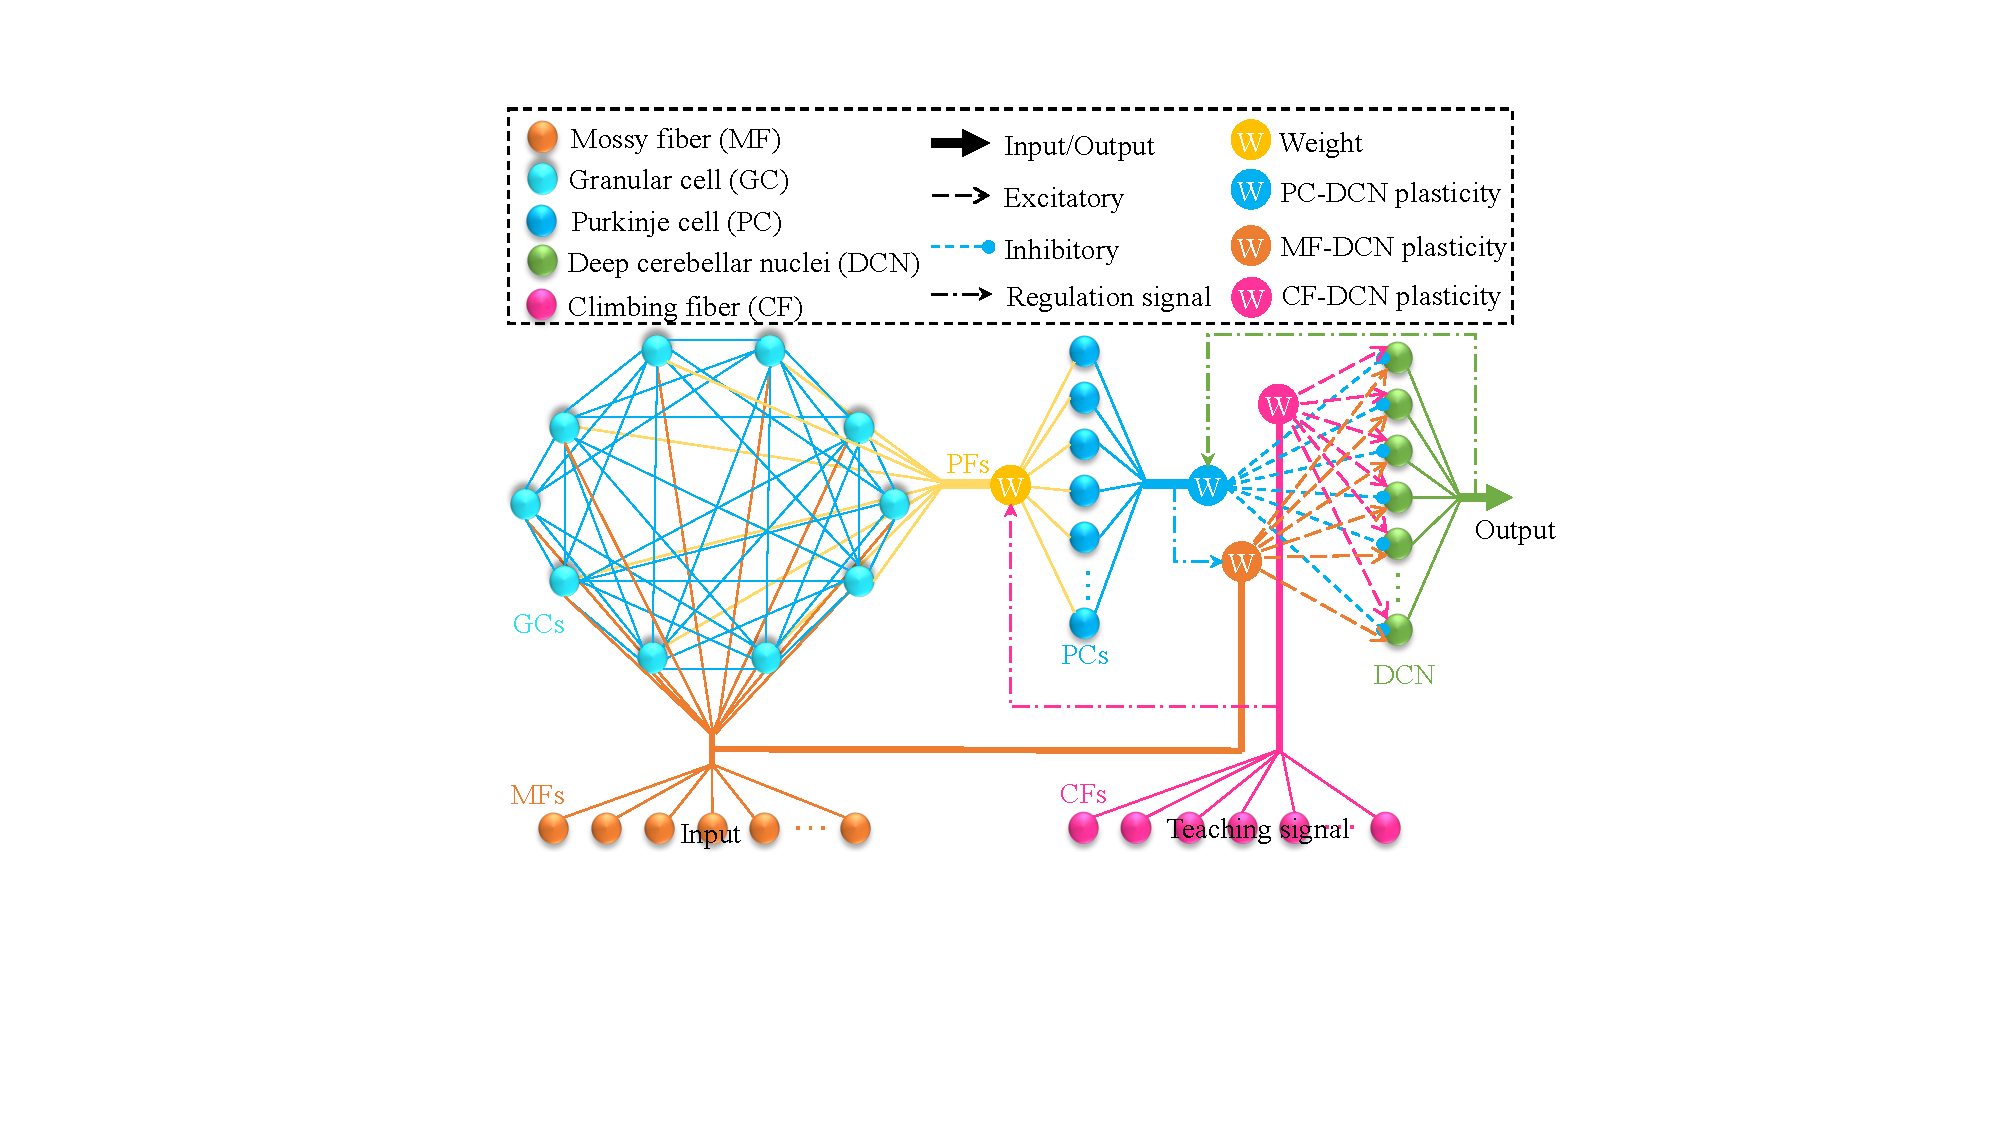
\includegraphics[width=0.8\linewidth]{figures/FIG1_TII-24-5492.pdf}
    \caption{Schematic diagram of the cerebellar neural network.
    }
    \label{Fig:Cerebellum}
\end{figure}
\subsection{Cerebellar Neural Network}

As shown in Fig.~\ref{Fig:Cerebellum}, the cerebellar neural network is mainly composed of five layers, namely mossy fibers (MFs), granular cells (GCs), Purkinje cells (PCs), climbing fibers (CFs), and deep cerebellar nuclei (DCN). The input layer (MFs) is responsible for conveying input signals of the cerebellum to internal layers. GCs process and encode the input signal in a manner similar to reservoir computing~\cite{Kalidindi2019}, which inspires us to utilize the echo state network~\cite{Jaeger2007} to replicate the function of GCs in this paper. The state of GCs is relayed by parallel fibers (PFs) and conveyed to PCs after being weighted. CFs carry error-related information, thus providing a teaching signal to the cerebellum. As the output layer, DCN responses to the integration of the inhibitory and excitatory contributed by MFs, PCs and CFs. The learning ability of the cerebellar neural network is highly related to the weight between PFs and PCs, and the synaptic plasticity among different layers.


\section{Methodology} \label{section:methodology}


\subsection{Problem Description}

Considering dual robotic manipulators, which are termed as the left manipulator and right manipulator respectively, we use vector forms, i.e. $\underline{q}_L(t)$ and $\underline{q}_R(t)$, of two dual quaternions to represent the end-effector poses of the two manipulators respectively. The desired poses of the manipulators are denoted by $\underline{q}_{d,L}(t)$ and $\underline{q}_{d,R}(t)$, which have different initial values but the same velocity. Our task is to ensure that not only the tracking error of a single manipulator but also the synchronization error between the two manipulators converge to zero. 

\subsection{Kinematics Learning}

The first step is to learn the uncertain kinematics of robotic manipulators. Since it is difficult to directly find the inverse of the mapping function $f$, the inverse kinematics (IK) problem is usually resolved at the velocity level with the aid of the Jacobian matrix $J$. In this part, we introduce how to learn Jacobian matrices. Firstly, inspired by~\eqref{eq:Jacobian}, the Jacobian initialization process of the left manipulator is as follows. Changing the angle of the $j$-th joint by an incremental amount $\Delta \theta_{L,j}$ independently, we can observe the effect of the $j$-th joint on the $i$-th dimension of the end-effector pose (i.e., end-effector displacement $\Delta \underline{q}_{L,i,j}$). Accordingly, the $(i,j)$-th element of the Jacobian matrix is initialized as $\tilde{J}_{L,i,j} = \Delta \underline{q}_{L,i,j}/\Delta \theta_{L,j}$ where $\tilde J$ denotes the estimated value of $J$. Because the specific value of the Jacobian matrix is related to the manipulator configuration, it is necessary to adapt the value of $\tilde J_L$ while operating. Inspired by~\eqref{eq:velKinematics}, the following norm-based energy function is defined
\begin{equation}
\xi_L= \frac{\|\dot{\underline{q}}_L - \tilde J_L \dot{\theta}_L\|_2^2}{2}
\end{equation}
where $\dot{\underline{q}}_L$ is the actual end-effector velocity of the left manipulator, $\dot{\theta}_L$ is the joint velocity of the left manipulator, $\tilde J_L \dot{\theta}_L$ can be deemed as estimated end-effector velocity, and $\|\cdot\|_2$ denotes the two-norm of a vector. Based on gradient descent, the adaptive law of the Jacobian matrix is designed as
\begin{equation}
\dot{\tilde J}_L = - \lambda \frac{\partial \|\dot{\underline{q}}_L - \tilde J_L \dot{\theta}_L\|_2^2}{\partial \tilde J_L} = \lambda \left(\dot{\underline{q}}_L - \tilde J_L \dot{\theta}_L\right)\dot{\theta}_L^{\rm T}
\label{eq:leftJacobianLearning}
\end{equation}
where $\dot{\tilde J}_L$ is the first time derivative of ${\tilde J}_L$, $\lambda>0$ is the convergence coefficient, and the superscript $(\cdot)^{\rm T}$ denotes transpose operation. The adaptation of the Jacobian matrix is performed online and relies on the real-time joint velocity and end-effector velocity. The joint velocity is provided by the controller and the end-effector velocity can be measured by sensors or estimated from pose data. Likewise, the Jacobian matrix of the right manipulator $\tilde J_R$ can be initialized and learned in the same way
\begin{equation}
\dot{\tilde J}_R = - \lambda \frac{\partial \|\dot{\underline{q}}_R - \tilde J_R \dot{\theta}_R\|_2^2}{\partial \tilde J_R} = \lambda \left(\dot{\underline{q}}_R - \tilde J_R \dot{\theta}_R\right)\dot{\theta}_R^{\rm T}.
\label{eq:rightJacobianLearning}
\end{equation}

Existing kinematics learning methods include offline data-driven approaches and online approaches. Compared to offline methods~\cite{Cursi2022RAL}, the gradient neurodynamic approach operates online and only requires sensory feedback data, allowing for rapid adaptation to different types of robotic systems. Although other online approaches also allow for rapid adaptation, the quadratic-programming-based approach suffers from low efficiency~\cite{Yip2016RAL}, and the zeroing-dynamics-based approach needs different feedback data~\cite{Yang2020}, including velocity and acceleration. In comparison, the gradient neurodynamic approach is computationally efficient and only needs velocity feedback.


\begin{figure*}[!t]
    \centering
    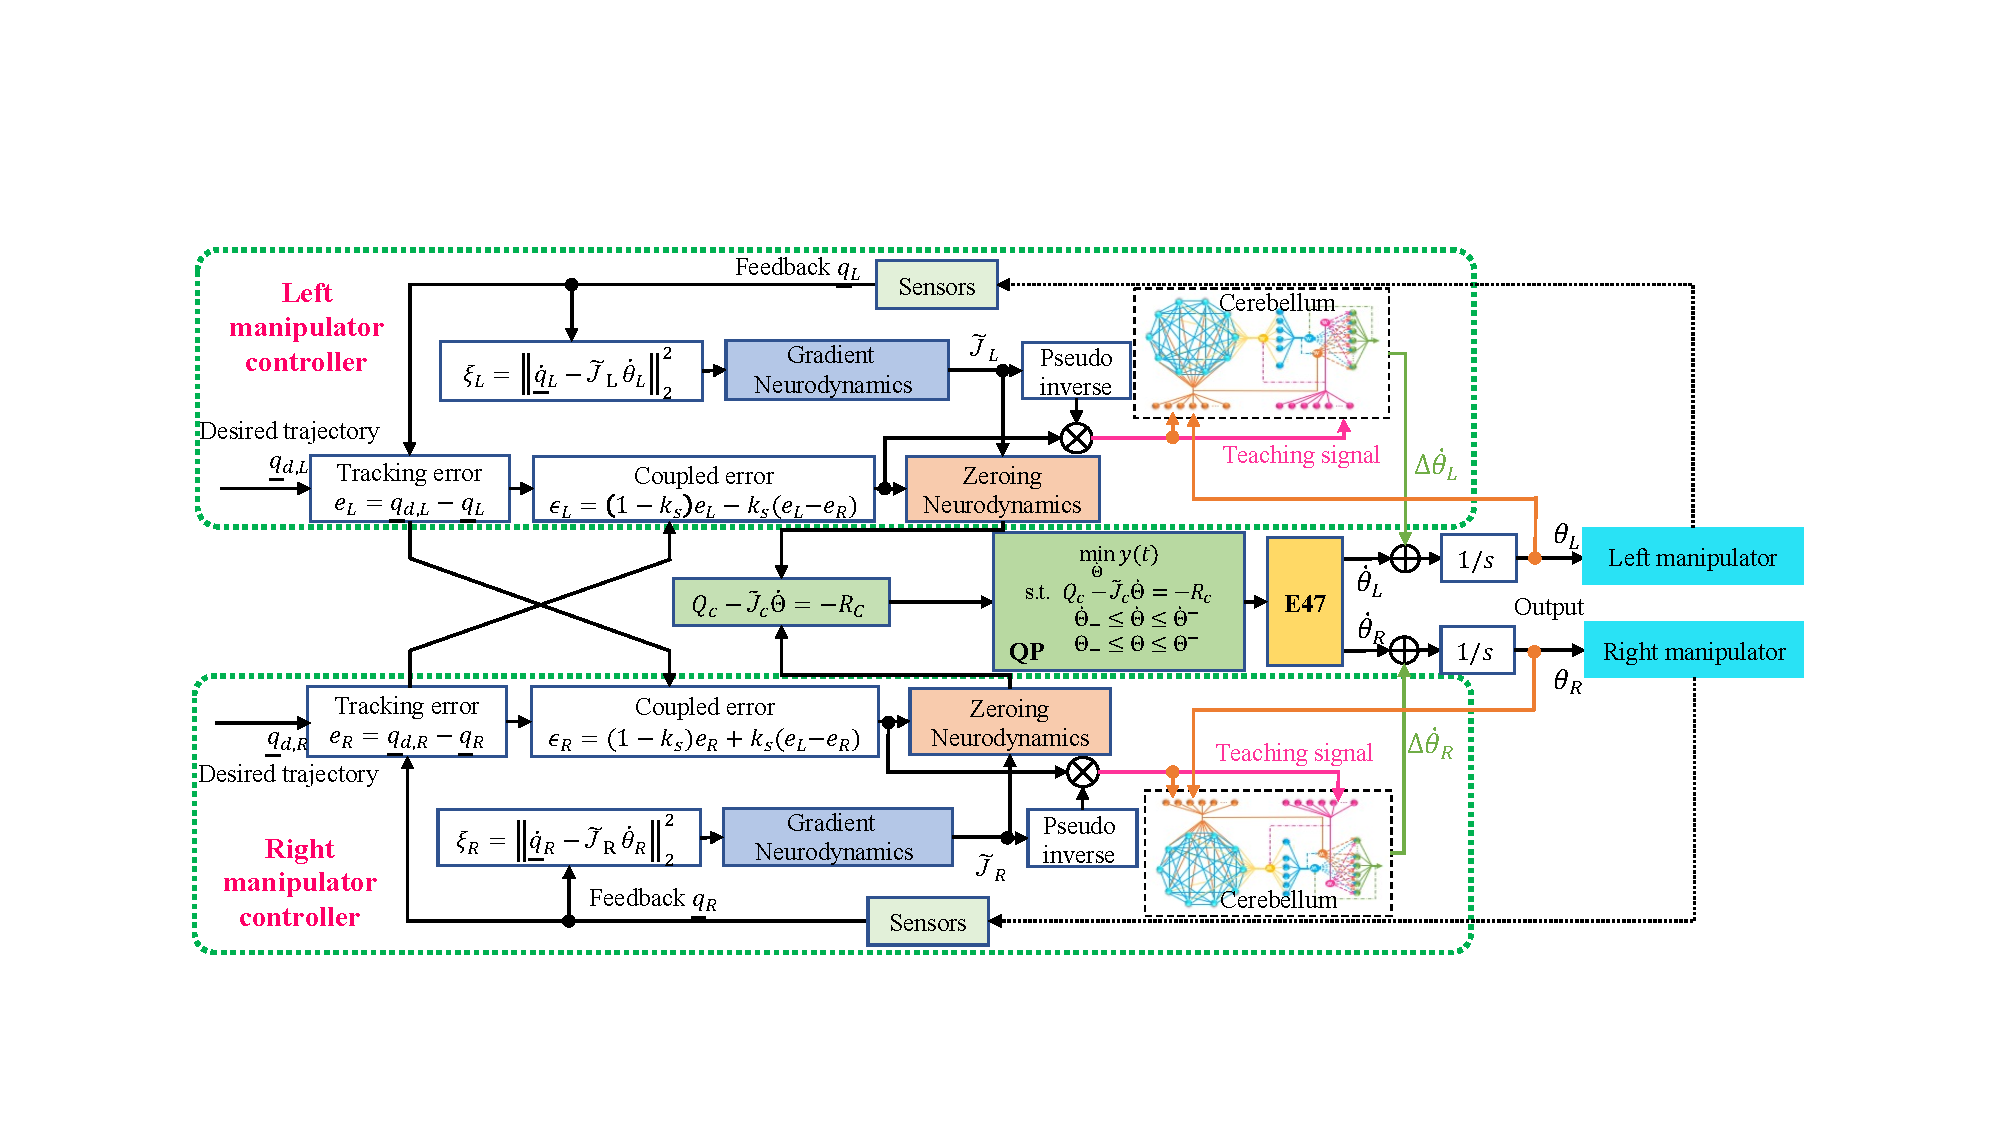
\includegraphics[width=0.9\linewidth]{figures/FIG2_TII-24-5492.pdf}
    \caption{Schematic diagram of the cerebellum-inspired synchronized tracking control method for dual robotic manipulators.
    }
    \label{Fig:KinematicController}
\end{figure*}

\subsection{Synchronized Tracking Control}

The tracking errors of the dual manipulators are defined as
\begin{equation}
\left\{\begin{aligned}
e_L = \underline{q}_{d,L} - \underline{q}_{L} \\
e_R = \underline{q}_{d,R} - \underline{q}_{R}
\end{aligned}\right.
\label{eq:tracking error}
\end{equation}
and the synchronization error is defined as
\begin{equation}
\varepsilon = e_L - e_R.
\end{equation}
Then, the coupled pose errors are defined as follows
\begin{equation}
\left\{\begin{aligned}
\epsilon_L = (1-k_s)e_L - k_s \varepsilon \\
\epsilon_R = (1-k_s)e_R + k_s \varepsilon
\end{aligned}\right.
\label{eq:coupled error}
\end{equation}
where $k_s \in [0,1)$, satisfying $k_s \ne \frac{1}{3}$, is the synchronization coefficient. When $k_s$ takes 0, the proposed control system will degrade to a distributed scheme, which cannot handle synchronization error, although the tracking task can be completed. By using the above coupled error, we can adjust the trade-off between the tracking error $e$ and the synchronization error $\varepsilon$ while avoiding the amplitude change of the overall coupled error, thereby avoiding the divergence problem caused by excessive feedback gain. The synchronized tracking control problem can be solved by forcing the coupled pose errors to converge to zero. This objective is achieved by resorting to the zeroing neurodynamic model~\cite{Zhang2015}, which is given by $\dot{\epsilon} = - \gamma \epsilon$, where $\epsilon$ denotes an error-monitoring function and $\gamma$ controls the convergence rate of the dynamic model. There are many methods that can solve the kinematic control problem of robotic manipulators, such as adaptive methods~\cite{Wang2020IFAC} and Jacobian pseudoinverse methods~\cite{Liao2015Robotica}. Compared to adaptive methods, the design procedure of the zeroing neurodynamic approach is more straightforward, avoiding complex theoretical analysis. Compared to traditional pseudoinverse methods, the zeroing neurodynamic approach has the potential to achieve better convergence and robustness by using nonlinear activation functions~\cite{Tan2022JAS}.

By exploiting the zeroing neurodynamic model, i.e., replacing the error-monitoring function $\epsilon$ with the coupled pose errors respectively, we have the following dynamic model
\begin{equation}\label{eq:dynamic model}
\left\{\begin{aligned}
\dot{\epsilon}_L = - \gamma \epsilon_L \\
\dot{\epsilon}_R = - \gamma \epsilon_R
\end{aligned}\right..
\end{equation}
Next, by expanding the above equation and replacing the Jacobian matrices with the learned ones, the following result is attained
\begin{equation}
\left\{\begin{aligned}
(1-2k_s)\left(\dot{\underline{q}}_{d,L} - \tilde{J}_L \dot{\theta}_L\right) +
k_s \left( \dot{\underline{q}}_{d,R} - \tilde{J}_R \dot{\theta}_R \right)
= -\gamma \epsilon_L \\
(1-2k_s)\left(\dot{\underline{q}}_{d,R} - \tilde{J}_R \dot{\theta}_R\right) +
k_s \left( \dot{\underline{q}}_{d,L} - \tilde{J}_L \dot{\theta}_L \right)
= -\gamma \epsilon_R 
\end{aligned}\right..
\end{equation}
For simplicity, the above equation can be written as the following compact form
\begin{equation}
Q_c - \tilde J_c \dot{\Theta} = -R_c
\label{eq:equality}
\end{equation}
where
\begin{equation}
Q_c = \left[\begin{matrix}
(1-2k_s)\dot{\underline{q}}_{d,L} + k_s \dot{\underline{q}}_{d,R} \\
(1-2k_s)\dot{\underline{q}}_{d,R} + k_s \dot{\underline{q}}_{d,L}
\end{matrix}\right],
\dot{\Theta} = \left[\begin{matrix}
\dot{\theta}_L \\
\dot{\theta}_R
\end{matrix}\right],
\end{equation}
\begin{equation}
\tilde J_c = \left[\begin{matrix}
&(1-2k_s) \tilde J_L & k_s \tilde J_R\\
& k_s \tilde J_L & (1-2k_s) \tilde J_R
\end{matrix}\right], 
R_c = \left[\begin{matrix}
\gamma \epsilon_L\\
\gamma \epsilon_R
\end{matrix}\right].
\end{equation}
Finally, the bimanual synchronized tracking control problem can be formulated as the quadratic programming (QP) problem
\begin{equation}
\begin{aligned}
\min_{\dot{\Theta}} y(t) = &\dot{\Theta}^\mathrm{T} W_q \dot{\Theta} + (\Theta(t)-\Theta(0))^\mathrm{T} \dot{\Theta} \\
\text{s.t.  } & Q_c - \tilde J_c \dot{\Theta} = -R_c \\
& \dot{\Theta}_- \le \dot{\Theta} \le \dot{\Theta}^- \\
& \Theta_- \le \Theta \le \Theta^-
\end{aligned}
\label{eq:QP}
\end{equation}
where $W_q$ is the identity matrix, $\Theta(0)$ denotes the initial joint angles of the dual manipulators, $\dot{\Theta}_-$ and $\Theta_-$ represent the lower bounds of joint velocities and joint angles respectively, $\dot{\Theta}^-$ and $\Theta^-$ represent the upper bounds of joint velocities and joint angles respectively. As shown in the QP scheme, the equality constraint guarantees that the two robots accurately track the desired trajectories. The design of the objective function $y(t)$ could bring other advantages, such as avoiding instability and joint angular drift~\cite{Zhang2004TSMC}, which is a common practice. By solving the QP problem~\eqref{eq:QP}, we can obtain the required joint velocity command. 

There are two differences between the proposed QP scheme and existing QP schemes. First, existing coordinated kinematic control methods are distributed~\cite{Zhang2021TNNLS,Jia2020Robotica,Zhan2024TNNLS}, which established QP schemes for each robot separately and neglected the synchronization error. In comparison, the proposed QP scheme is centralized and incorporates the synchronization constraint. Second, most existing QP-based coordinated control methods have considered position control but ignored orientation control~\cite{Zhang2021TNNLS,Jia2020Robotica,Zhan2024TNNLS}. In comparison, this work can achieve the position and orientation control simultaneously. Unlike previous non-QP approaches that require two separate models to handle position and orientation respectively~\cite{YANG2021108007}, our method unifies both aspects within a single model by using the dual quaternion. This leads to a more streamlined and compact inverse kinematics solution.


A lot of methods have been proposed to solve QP problems~\cite{Xia20204TMTCI}. As one of the solutions to QP problems, the E47 algorithm~\cite{Zhang2011} has high accuracy and fast convergence. More importantly, it is suitable for the solution of QP problems involving high-DOF robotic manipulators. Although recurrent neural network (RNN) methods are computationally efficient for solving QP problems~\cite{Jia2020Robotica,Liu2022b}, they require small sampling intervals of time (e.g., 0.001 s). However, we have to choose larger sampling intervals (e.g., 0.1 s) because of the hardware limitation in physical experiments. In this situation, the accuracy of RNN methods cannot meet the requirement, while the E47 algorithm can achieve much higher accuracy. Therefore, we employ the E47 algorithm to solve the QP problem~\eqref{eq:QP} in this paper. The solution to the QP problem needs to be iteratively calculated at each time step. At the $k$-th time step, given an initial solution $s_0$, for the iteration index $j = 0,1,2,\cdots$, the following E47 iteration formula is utilized to find the optimal solution
\begin{equation}
 s_{j+1} = \Omega\left( s_j - \rho( s_j) d( s_j)\right)
 \label{eq:QP solver}
\end{equation}
where
\begin{equation}
\begin{aligned}
 & e( s_j)  =  s_j - \Omega( s_j -( M  s_j +  z)),\\
 & d( s_j)  = (M^T +  I) e( s_j), 
 \rho( s_j) = \frac{\|e( s_j)\|_2^2}{\|d(s_j)\|_2^2} \label{eq: rho}
\end{aligned}
\end{equation}
with $\|\cdot\|_2^2$ denoting the square of the two-norm of a vector, $\Omega$ being a projection to the set of feasible solution, and
\begin{equation}
M = \left[\begin{matrix}
I &- \tilde{J}_c^\mathrm{T} \\ 
\tilde{J}_c & 0
\end{matrix}\right], z=\left[\begin{matrix}
\Theta(t)-\Theta(0) \\ 
Q_c + R_c
\end{matrix}\right].
\end{equation}
In particular, we assume that the optimal solution at the $k$-th time step is found if $\|e(s_j)\|_2 $ is less than a sufficient small constant. Then, the first $n_L+n_R$ elements of $s_j$ constitute the solution to~\eqref{eq:QP}, where $n_L$ and $n_R$ are the numbers of joints of the dual manipulators respectively.

\begin{remark}
When solving the QP scheme~\eqref{eq:QP}, it can be ensured that the equality~\eqref{eq:equality} (i.e., zeroing neurodynamic model) holds. Existing studies have proven and validated that the zeroing neurodynamic model is able to force its state function to converge to zero~\cite{Tan2022JAS}, i.e., $\epsilon_L \to 0$ and $\epsilon_R \to 0$. When $\epsilon_L=0$ and $\epsilon_R=0$, we have $\epsilon_L-\epsilon_R=\left(1-3k_s\right)\varepsilon=0$, which means $\varepsilon=0$ if $k_s \ne \frac{1}{3}$. Therefore, by choosing $k_s$ from the range $\left(0,\frac{1}{3}\right)$ or $\left(\frac{1}{3},1\right)$, zeroing neurodynamic models can force the synchronization error $\varepsilon$ to converge to 0, thereby ensuring that there will be no large synchronization errors.
\end{remark}



\begin{algorithm}[tbp]
  \caption{Description of the proposed bimanual synchronized tracking control method for dual robotic manipulators.}
  \begin{algorithmic}[1]
    \STATE Parameter setting: $k_s,\lambda,\gamma,k_l, k_g,\eta, \alpha, T_d$.
    \STATE Initialize Jacobian matrices $\tilde{J}_L,\tilde{J}_R$.
    \FOR{$t\in[0,T_d]$}
      \STATE Measure end-effector poses $\underline{q}_L$ and $\underline{q}_R$  by sensors.
      \STATE Determine tracking errors $e_L,e_R$ based on~\eqref{eq:tracking error} and coupled errors $\epsilon_L, \epsilon_R$ based on~\eqref{eq:coupled error}.
      \STATE Formulate the QP scheme~\eqref{eq:QP}.
      \STATE Solve the QP problem using the E47 algorithm to get joint velocities $\dot{\theta}_L$ and $\dot{\theta}_R$. 
      \STATE Determine the input $\chi^{MF}_L=[\theta_L; \zeta_L]$ and teaching signal $\chi^{CF}_L=\zeta_L$ for the cerebellum model of the left manipulator, and the input $\chi^{MF}_R=[\theta_R; \zeta_R]$ and teaching signal $\chi^{CF}_R=\zeta_R$ for the cerebellum model of the right manipulator.
      \STATE Cerebellum forward propagation: \\
            \eqref{eq:GC} $\to \chi^{GC}$, \eqref{eq:PC} $\to \chi^{PC}$, \eqref{eq:DCN} $\to \chi^{DCN}$, \\ 
            $\Delta \dot{\theta}_L = \chi^{DCN}_L$, $\Delta \dot{\theta}_R = \chi^{DCN}_R$.
      \STATE Cerebellum backward propagation: \\
            \eqref{eq:W PF-PC} $\to \Delta W^{PF-PC}$, \eqref{eq:W MF-DCN} $\to \Delta W^{MF-DCN}$, \\ 
            \eqref{eq:W PC-DCN} $\to \Delta W^{PC-DCN}$, \eqref{eq:W CF-DCN} $\to \Delta W^{CF-DCN}$, \\
            $W \doteq (1-\alpha) W + \alpha \Delta W$.
      \STATE Fine-tune joint velocities: \\
            $\dot{\theta}_L^\ast = \dot{\theta}_L + \Delta \dot{\theta}_L$, $\dot{\theta}_R^\ast = \dot{\theta}_R + \Delta \dot{\theta}_R$.
      \STATE Update Jacobian matrices: \eqref{eq:leftJacobianLearning} $\to \tilde{J}_L$, \eqref{eq:rightJacobianLearning} $\to \tilde{J}_R$.
      \STATE Control the robots with joint angles $\theta_L$ and $\theta_R$.
    \ENDFOR
  \end{algorithmic}
  \label{algorithm:CI-SyncTC}
\end{algorithm}

\begin{figure*}[!t]
    \centering
    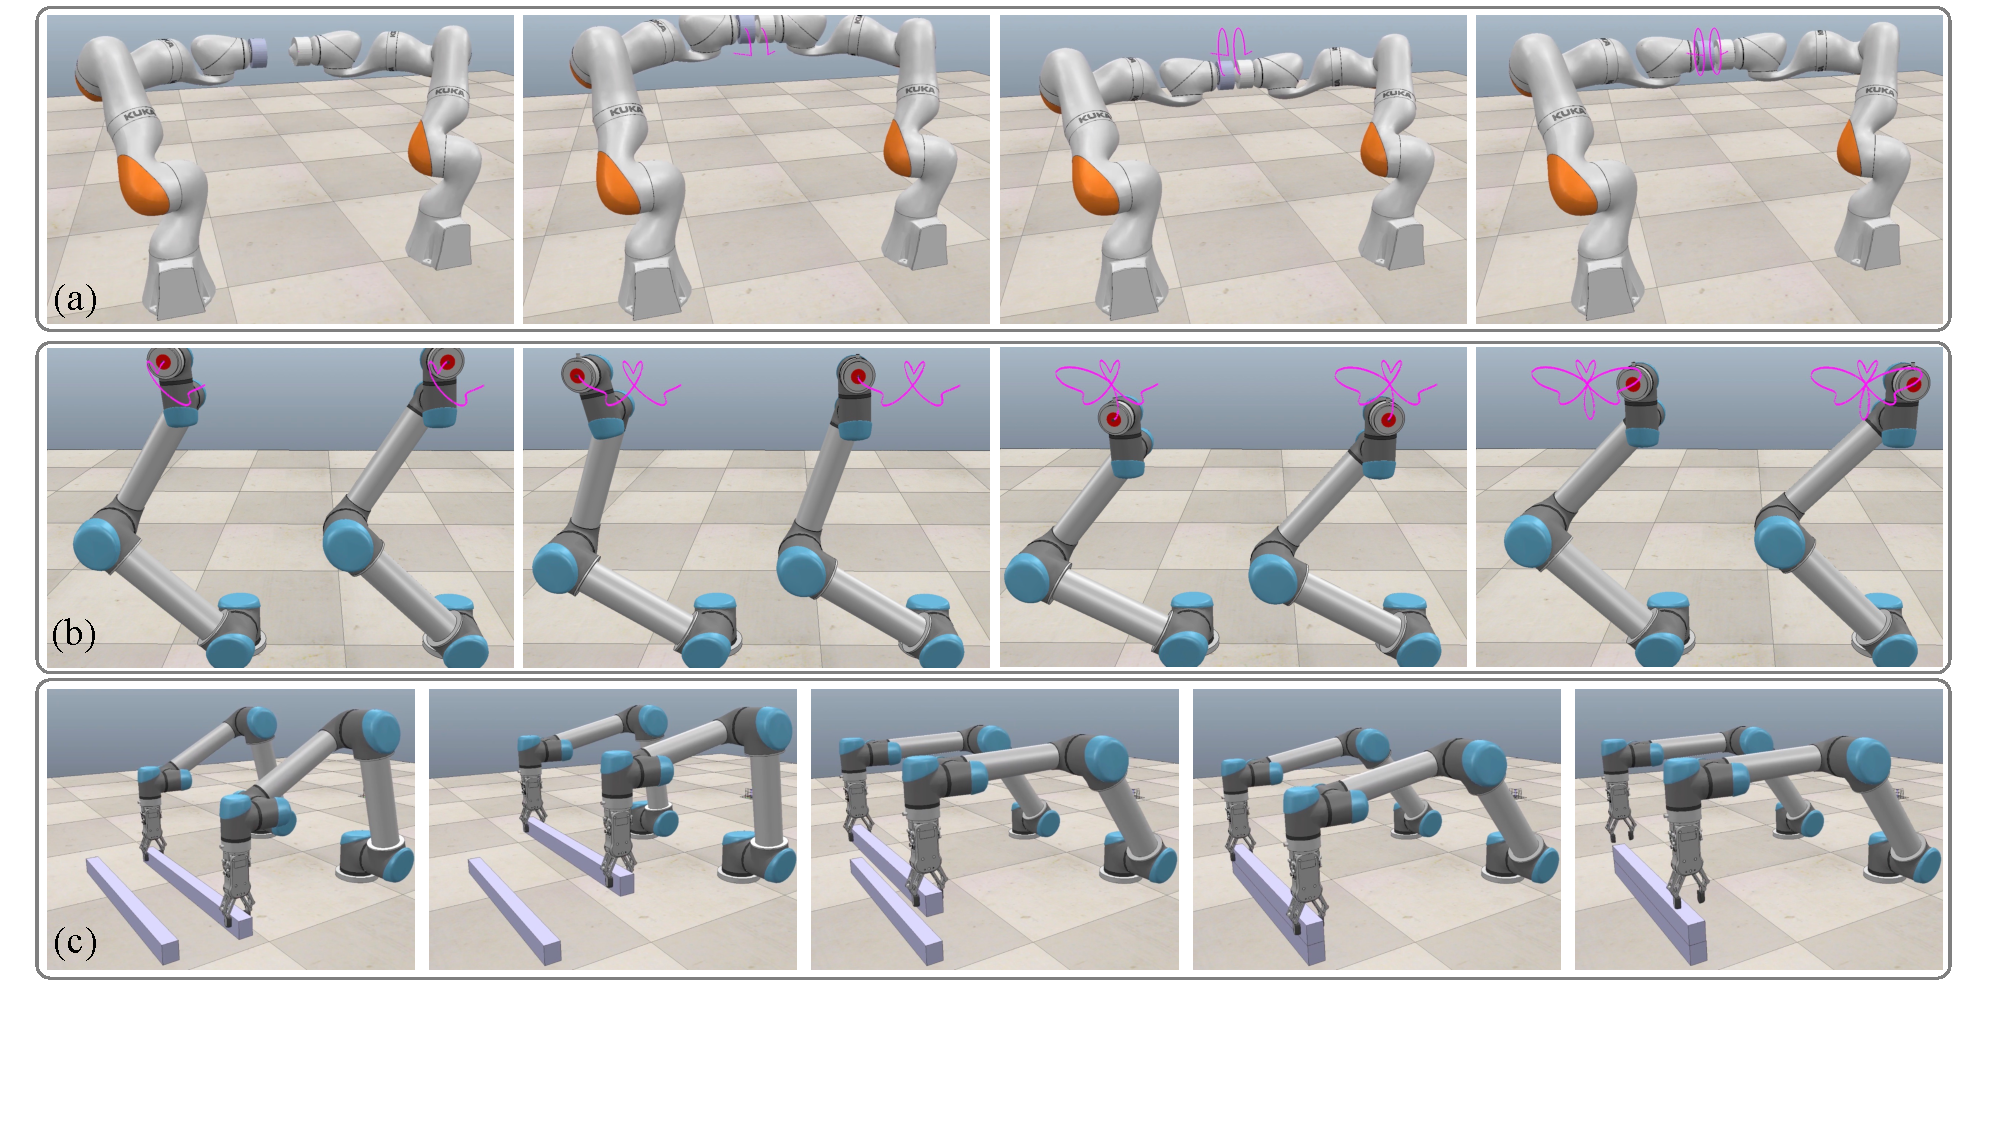
\includegraphics[width=0.9\linewidth]{figures/simulation/FIG3_TII-24-5492.pdf}
    \caption{Snapshots of simulations in V-REP. (a) Dual KUKA manipulators track circular trajectories synchronously. (b) Dual UR5 manipulators track butterfly trajectories synchronously. (c) Application of the proposed control system to a coordinated transportation task.
    }
    \label{Fig:sim:circularPathSnapshots}
\end{figure*}

\subsection{Cerebellum-Inspired Control}

In this part, we endow the control system with learning ability by introducing a cerebellar neural network. To the best of the authors' knowledge, existing coordinated kinematic control methods for dual robotic manipulators only adopt traditional numerical methods~\cite{Chen2020,Zhang2021TNNLS}. Compared to these methods, using cerebellum-inspired control technique can equip the control system with continuous learning capability, thereby achieving better accuracy. The input to the network (i.e., the state of the MFs layer) is denoted by the vector $\chi^{MF}$. The continuous-time dynamics of the GCs layer is as follows
\begin{equation}
k_g\dot{\chi}^{GC} = (1-k_l) \chi^{GC} + \psi\left(W^{MF-GC}\chi^{MF} + W^{GC} \chi^{GC}\right)
\label{eq:GC}
\end{equation}
where $\chi^{GC}$ is a vector representing the state of the GCs layer, $W^{MF-GC}$ is the weight matrix between the MFs layer and the GCs layer, $W^{GC}$ is the internal weight matrix of the GCs layer, $k_g > 0$ denotes the speed of dynamics, $k_l \in [0,1]$ represents leakage rate, and $\psi(\cdot)$ is the sigmoid activation function. Both the weight matrices are set to random values. The PFs are used to relay the signal of the GCs layer, which means $\chi^{PF} = \chi^{GC}$. The state of the PCs layer is the weighted sum of the signal carried by the PFs layer
\begin{equation}
\chi^{PC} = \tanh\left(W^{PF-PC}\chi^{PF}\right)
\label{eq:PC}
\end{equation}
where $W^{PF-PC}$ is the output weight matrix and $\tanh(\cdot)$ is the activation function. The output weight matrix is initialized as zero and updated based on the covariance learning rule~\cite{Porrill2007}
\begin{equation}
\Delta W^{PF-PC} = \eta \chi^{CF} \left(\chi^{PF}\right)^{\rm T}
\label{eq:W PF-PC}
\end{equation}
where $\Delta W^{PF-PC}$ is the weight change, $\eta > 0$ is the learning rate and $\chi^{CF}$ is the teaching signal provided by the CFs layer. In addition to the output weight $W^{PF-PC}$, the synaptic plasticity among different layers also plays an important role in the learning process of the cerebellar neural network. There are three different forms of synaptic plasticity in the cerebellar neural network. During the learning process, the synaptic strengths are adapted progressively based on the following synaptic plasticity mechanisms~\cite{Tolu2020}:
\begin{itemize}
\item The MF-DCN synaptic plasticity is updated as
\begin{equation}
\Delta W_{i}^{MF-DCN} = \frac{\text{LTP}_{\max}}{|\chi_i^{PC}|+1} - \text{LTD}_{\max} \chi^{PC}_i
\label{eq:W MF-DCN}
\end{equation}
where the vector $W^{MF-DCN}$ denotes the synaptic strength between the MFs layer and the DCN layer, $\Delta W_{i}^{MF-DCN}$ denotes the change of the $i$-th element of the vector, $|\chi^{PC}_i|$ is the absolute value of the $i$-th element of $\chi^{PC}$, $\text{LTP}_{\max} = 0.001$ and $\text{LTD}_{\max}=-0.01$ are the maximum long term potentiation/depression (LTP/LTD).
\item The PC-DCN synaptic plasticity is updated as
\begin{equation}
\Delta W_{i,i}^{PC-DCN} = \frac{\text{LTP}_{\max}|\chi_i^{PC}|}{|\chi_i^{DCN}|+1} - \text{LTD}_{\max} (1-|\chi^{PC}_i|)
\label{eq:W PC-DCN}
\end{equation}
where the diagonal matrix $W^{PC-DCN}$ denotes the synaptic strength between the PCs layer and the DCN layer, $\Delta W_{i,i}^{PC-DCN}$ denotes the change of the $(i,i)$-th element of the matrix, $\chi^{DCN}$ is a vector representing the state of DCN layer, $\text{LTP}_{\max} = 0.001$ and $\text{LTD}_{\max}=0.01$ are the maximum LTP/LTD.
\item The CF-DCN synaptic plasticity is updated as
\begin{equation}
\Delta W_{i,i}^{CF-DCN} = \text{MTP}_{\max} |\chi^{CF}_i|- \frac{\text{MTD}_{\max}}{|\chi_i^{CF}|+1}
\label{eq:W CF-DCN}
\end{equation}
where the diagonal matrix $W^{CF-DCN}$ denotes the synaptic strength between the CFs layer and the DCN layer, $\Delta W_{i,i}^{CF-DCN}$ denotes the change of the $(i,i)$-th element of the matrix, $\text{MTP}_{\max}=0.001$ and $\text{MTD}_{\max}=-0.01$ are the maximum modulating term potentiation/depression (MTP/MTD).
\end{itemize}


Typically, the DCN layer is inhibited by PCs, and excited by MFs and CFs. Therefore, the output of the cerebellar neural network (i.e., the state vector of DCN layer) is described as
\begin{equation}
\chi^{DCN} = W^{MF-DCN} + W^{CF-DCN}\chi^{CF} - W^{PC-DCN}\chi^{PC}.
\label{eq:DCN}
\end{equation}
The synaptic strength matrices are updated via $W \doteq (1-\alpha)W + \alpha \Delta W$ where $\alpha \in [0,1]$ is the update factor. Finally, we fine-tune the proposed synchronized kinematic tracking controller with the cerebellar neural network. Specifically, we deploy two cerebellar neural networks for the dual manipulators respectively. The inputs to cerebellar neural networks are joint angles and estimated joint-space errors. The error-related signals are taken as teaching signals of cerebellar neural networks. For example, for the left manipulator, the task-space coupled error $\epsilon_L$ is transformed to the joint-space error by the learned Jacobian matrix as $\zeta_L = \tilde J_L^\dag \epsilon_L$, where $\tilde J_L^\dag$ is the pseudo inverse of $\tilde J_L$. The joint-space error $\zeta_L$ is the teaching signal of the cerebellar neural network for the left manipulator. The outputs of cerebellar neural networks are used to fine-tune the joint velocity command $\dot{\Theta}$, which is obtained by solving the QP problem. By integrating the modified joint velocity command, we can obtain the joint angle command. For ease of understanding, the schematic diagram of the proposed bimanual cerebellum-inspired synchronized kinematic tracking controller for dual manipulators is depicted in Fig.~\ref{Fig:KinematicController}. Besides, the algorithm description of the proposed control system is elaborated in Algorithm~\ref{algorithm:CI-SyncTC}.



\section{Simulations and Experiments} \label{section:experiment}


\subsection{Simulations}

In this part, simulations are performed on the virtual robot experimentation platform (V-REP). The synchronization coefficient is set as $k_s= 0.1$. The convergence coefficient for kinematics learning is set as $\lambda = 0.5$. The convergence rate of the zeroing neurodynamic model is chosen as $\gamma = 2$. For the cerebellar neural network, the number of GCs is $400$, the leakage rate is $k_l = 0.6$, the speed of the dynamics is $k_g = 0.5$, and the learning rate $\eta$ is set to $0.001$. Three dual-manipulator platforms are built in V-REP as shown in Fig.~\ref{Fig:sim:circularPathSnapshots}. In the first platform, two modules are attached to the end-effector of the dual KUKA R800 manipulators respectively. To verify the feasibility of the proposed cerebellum-inspired synchronized tracking control (CI-SyncTC) method, our first task is to control the dual KUKA manipulators to align the modules and move them along circular trajectories synchronously while maintaining the module orientation unchanged.


\begin{figure}[!t]
    \centering
    \subfigure[]{
    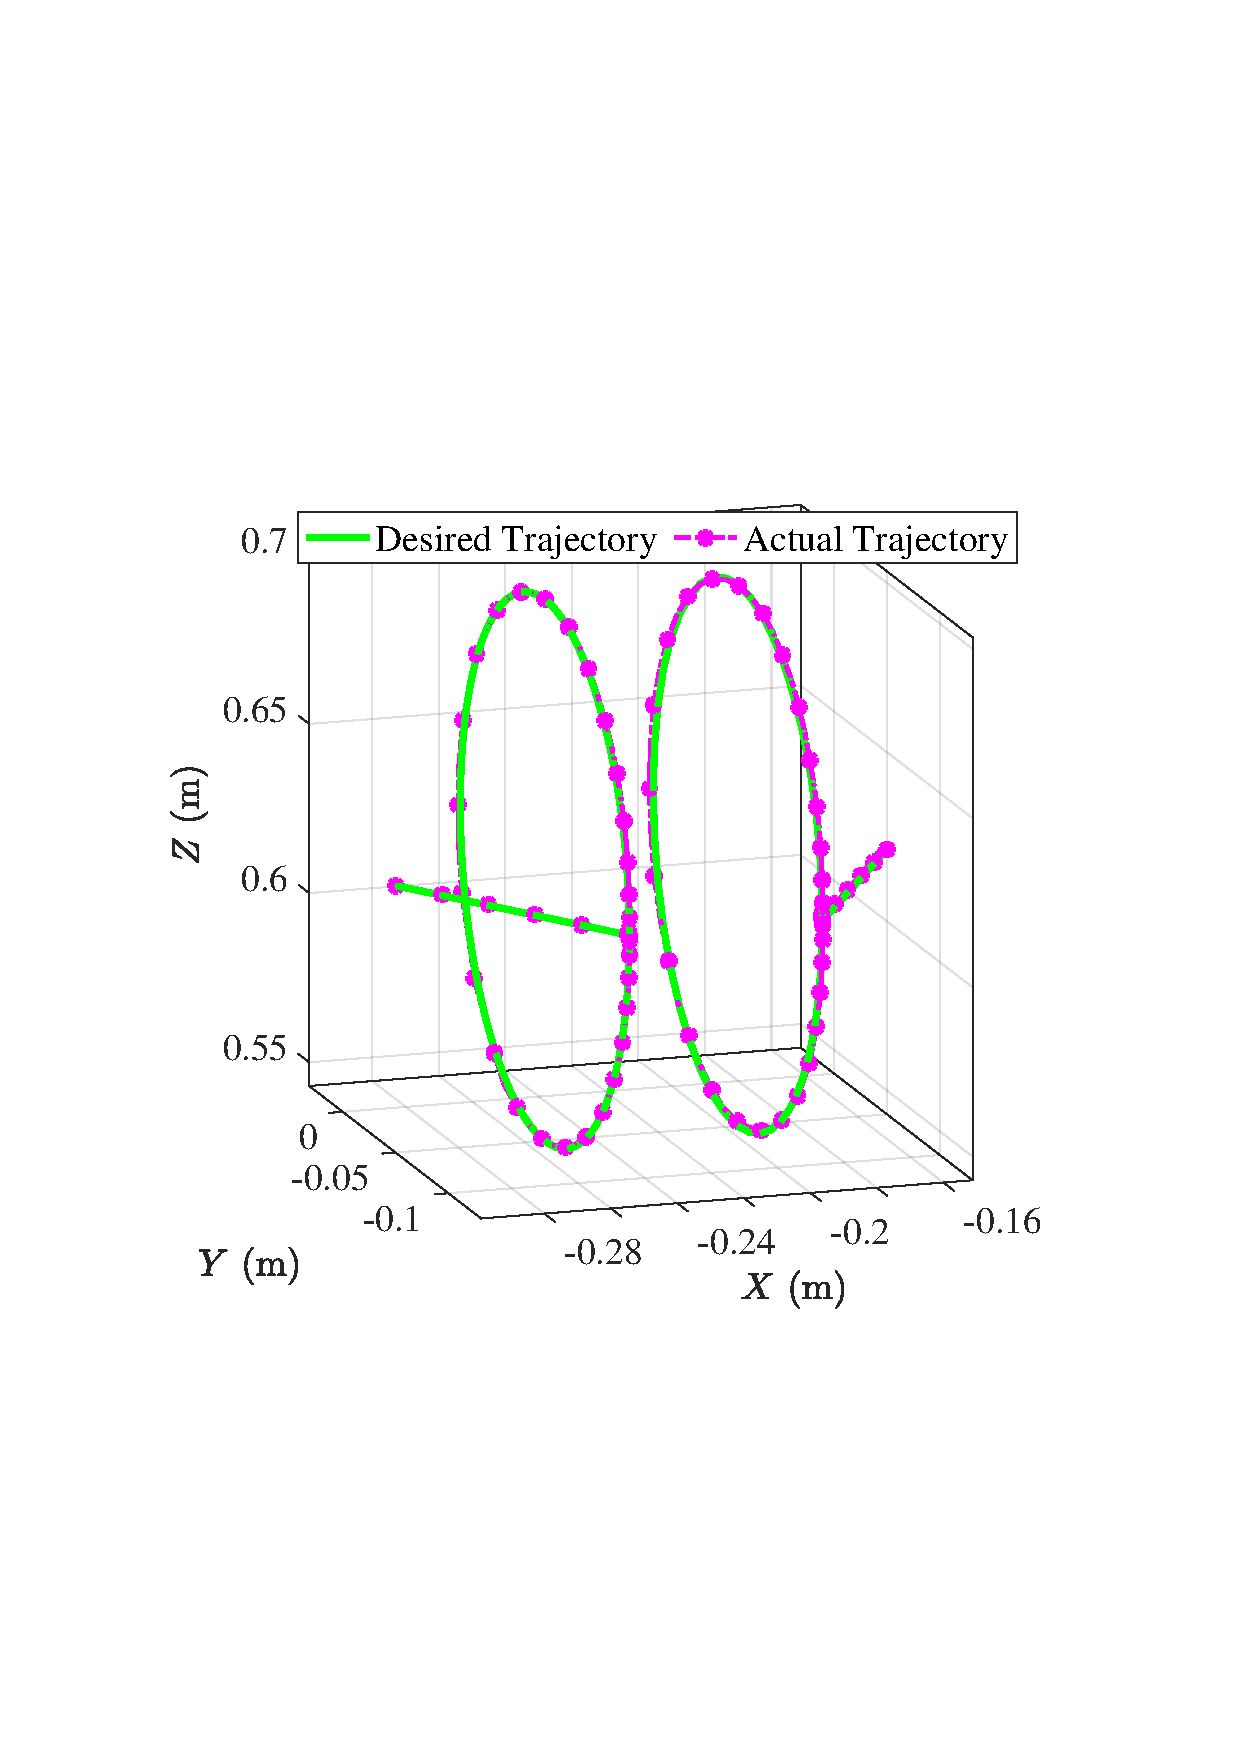
\includegraphics[width=0.4\linewidth]{figures/simulation/FIG4a_TII-24-5492.pdf}
    \label{figures:simulation:path comparison:a}
    }
    \subfigure[]{
    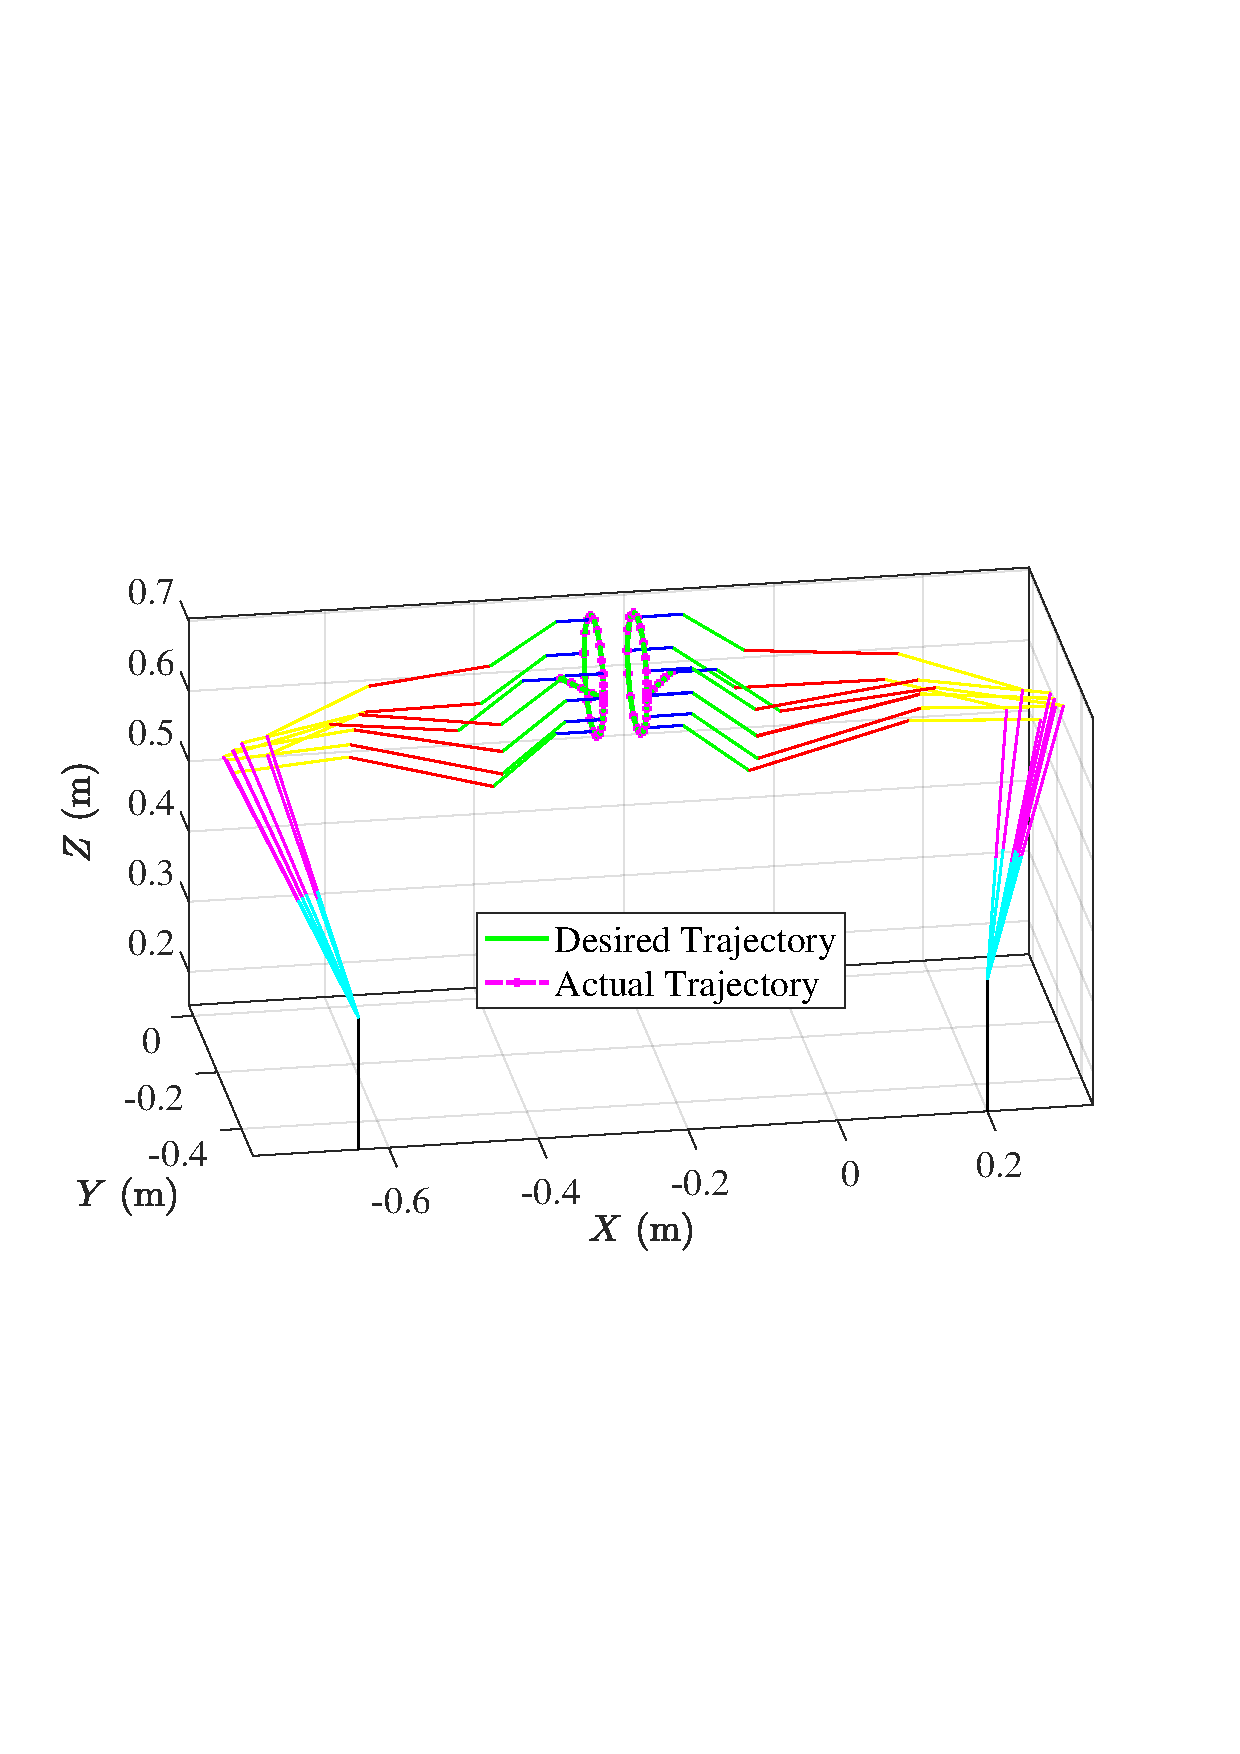
\includegraphics[width=0.52\linewidth]{figures/simulation/FIG4b_TII-24-5492.pdf}
    \label{figures:simulation:path comparison:b}
    }
    \caption{Trajectories of the dual KUKA manipulators. (a) Comparison between the desired end-effector trajectories and the actual trajectories. (b) Illustration of robot trajectories.
    }
    \label{figures:simulation:path comparison}
\end{figure}

\begin{figure}[!t]
    \centering
    \subfigure[]{
        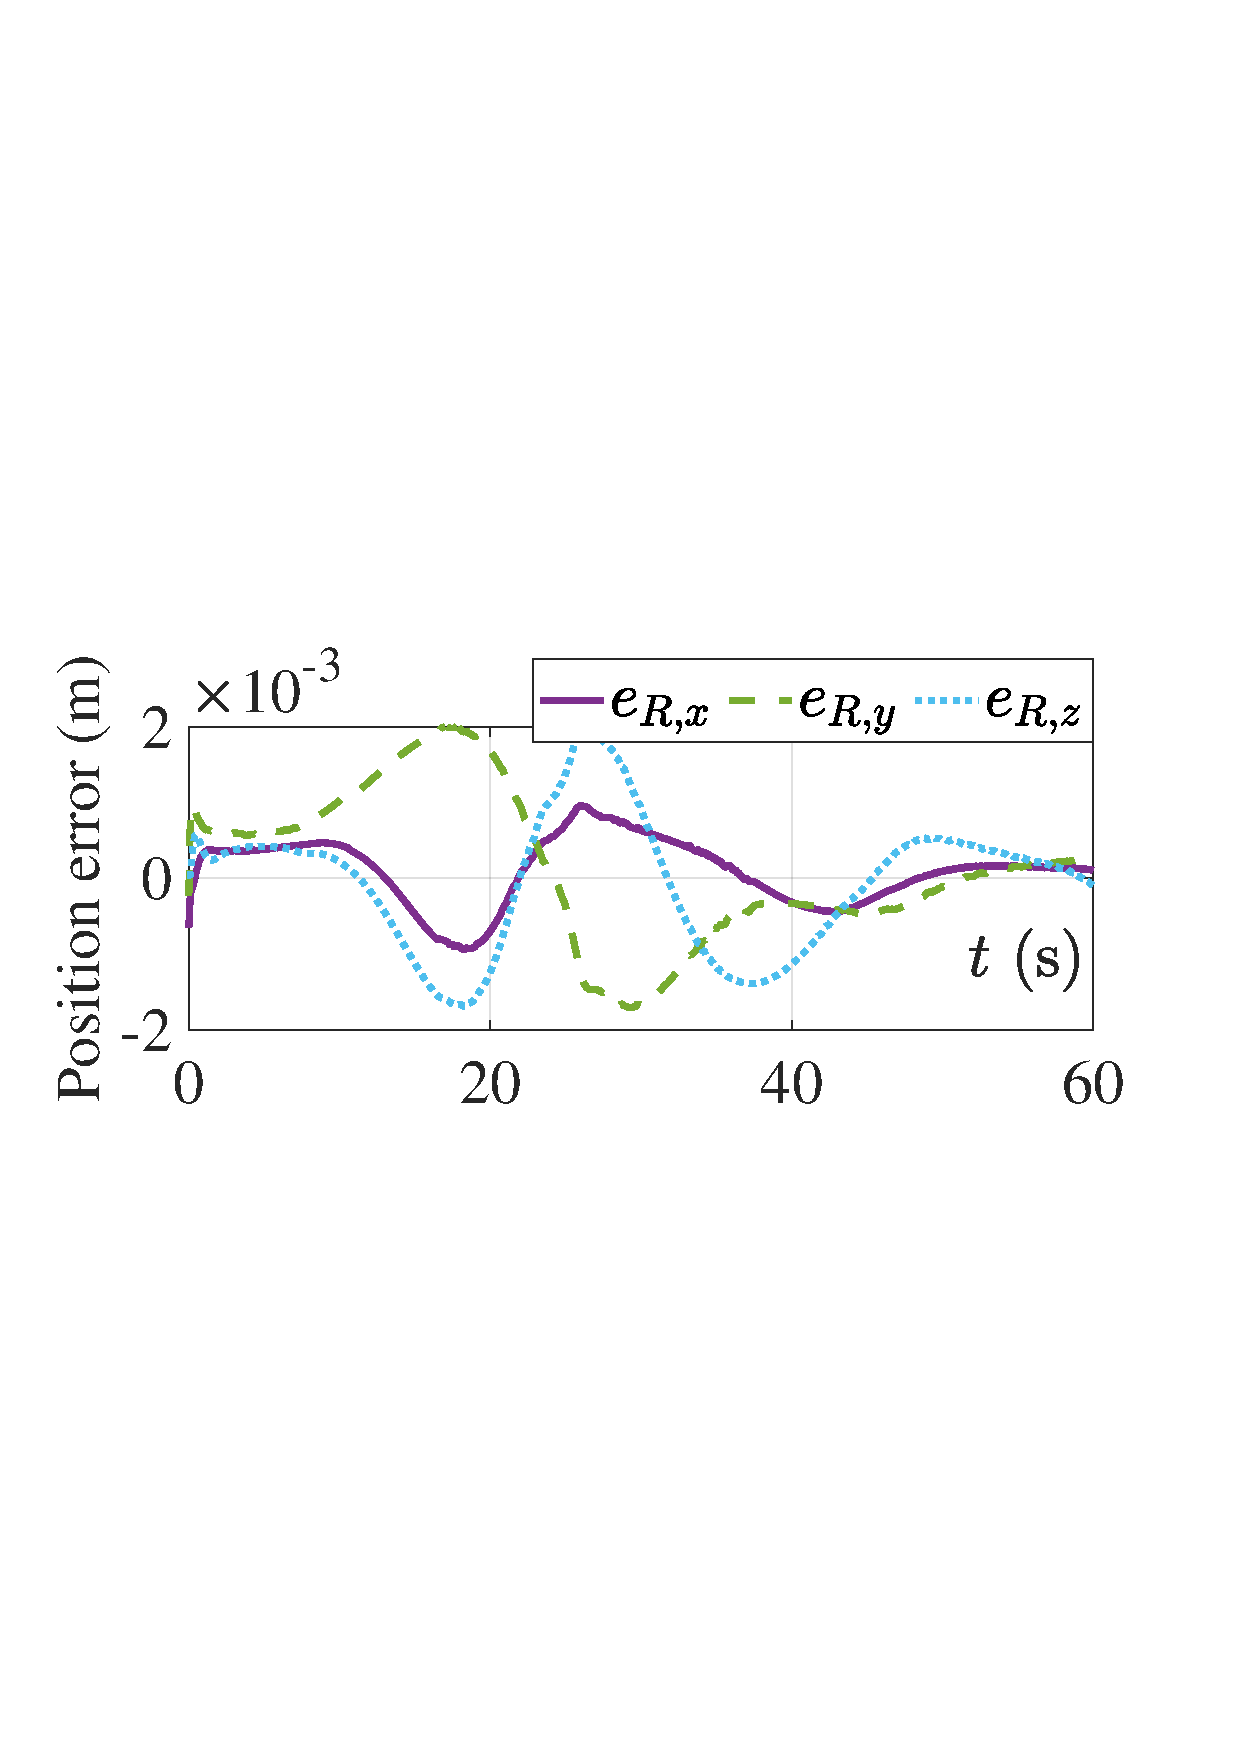
\includegraphics[width=0.45\linewidth]{figures/simulation/FIG5a_TII-24-5492.pdf}
        \label{figures:simulation:circle tracking results:a}
    }
    \hspace{0in}
    \subfigure[]{
        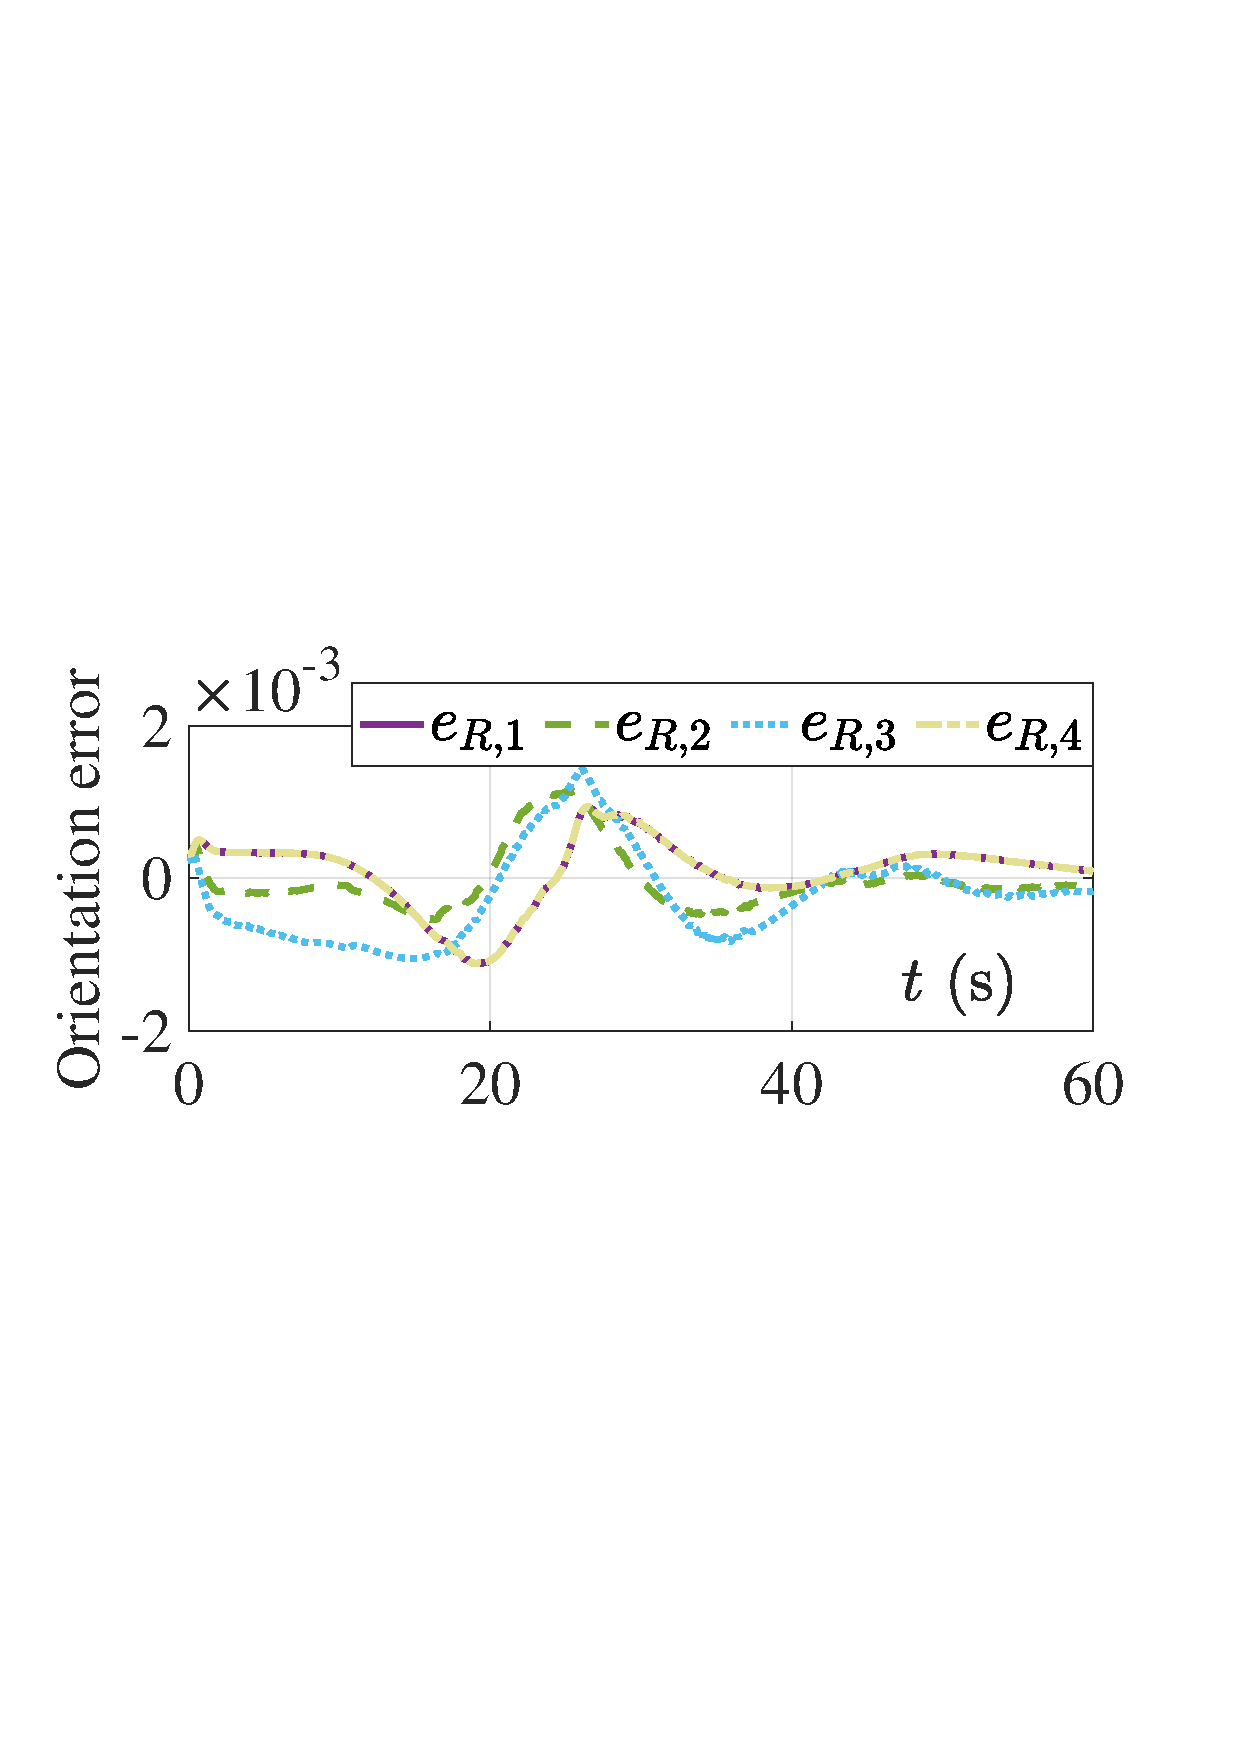
\includegraphics[width=0.45\linewidth]{figures/simulation/FIG5b_TII-24-5492.pdf}
        \label{figures:simulation:circle tracking results:b}
    }
    \hspace{0in}
    \subfigure[]{
        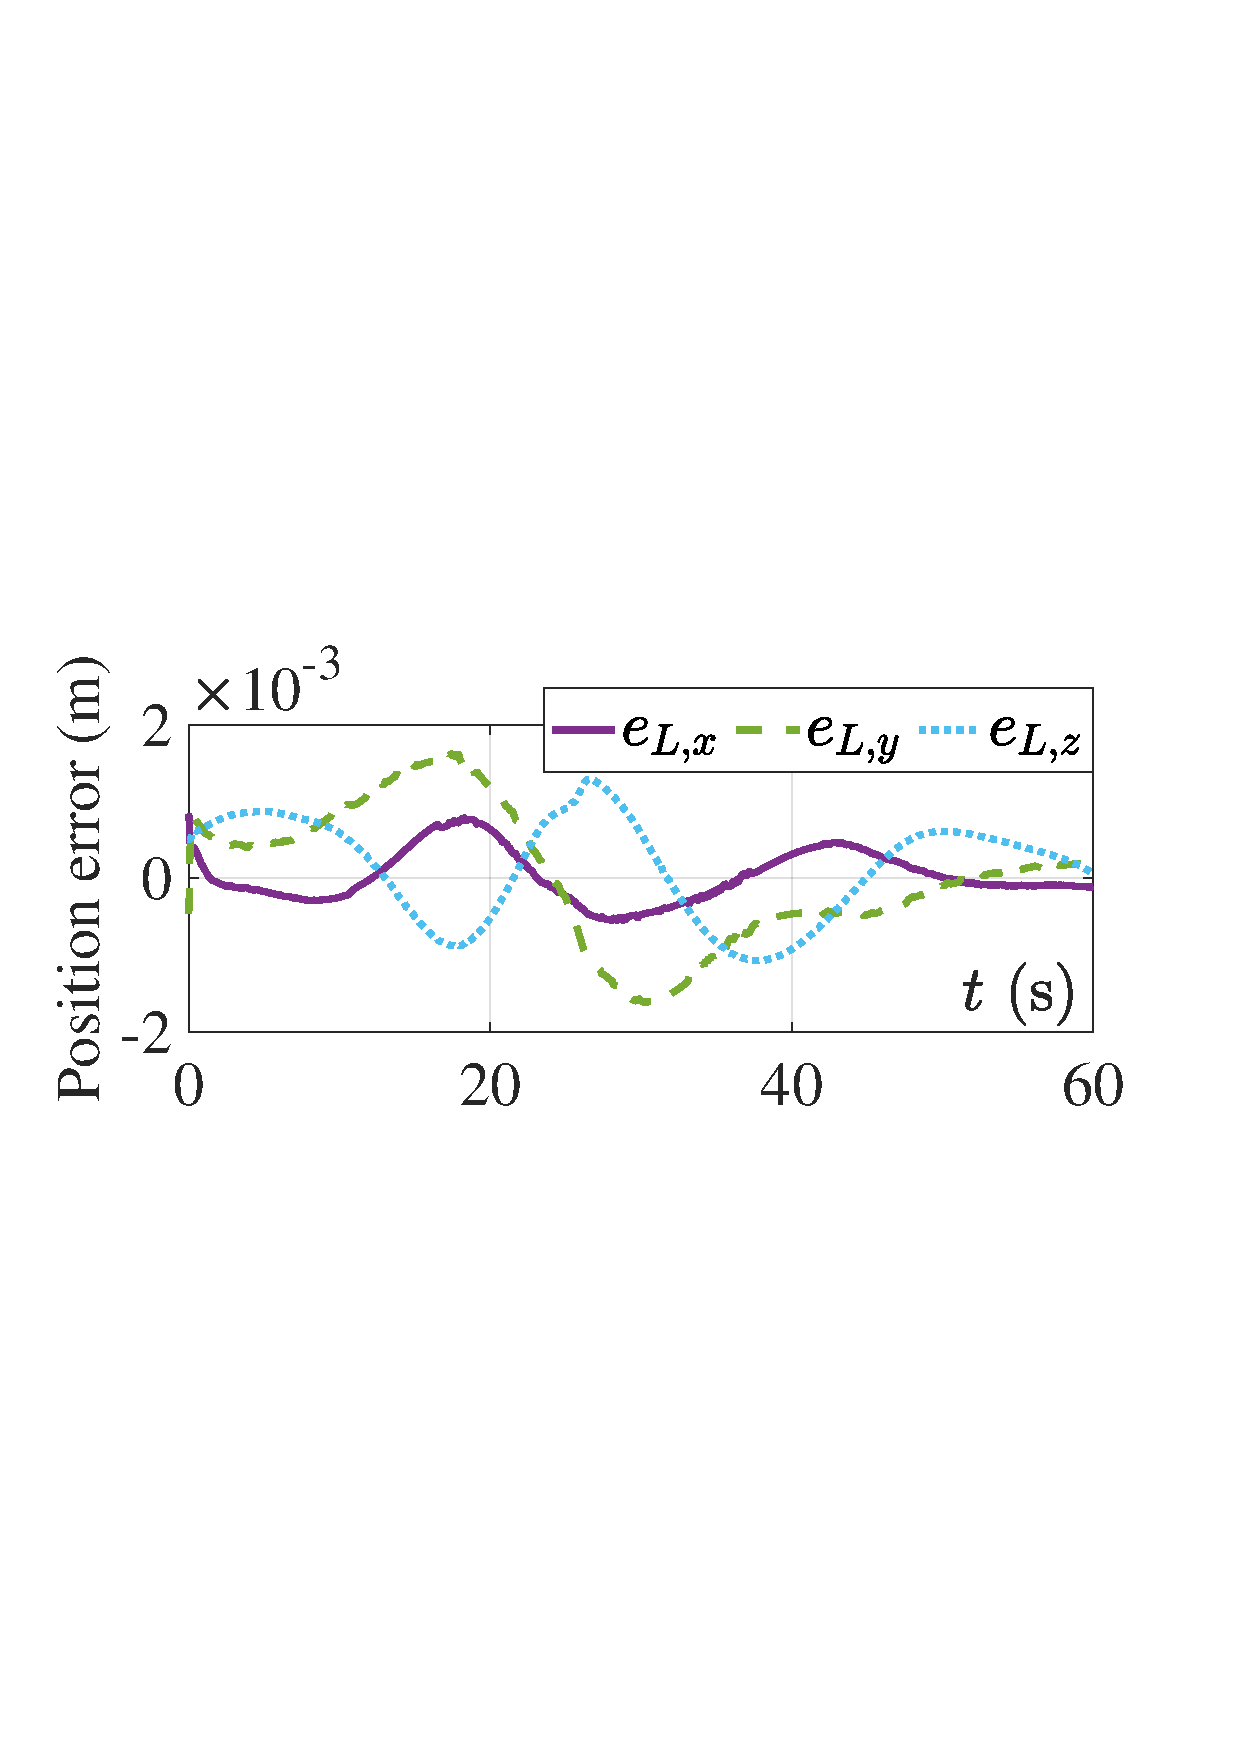
\includegraphics[width=0.45\linewidth]{figures/simulation/FIG5c_TII-24-5492.pdf}
        \label{figures:simulation:circle tracking results:c}
    }
    \hspace{0in}
    \subfigure[]{
        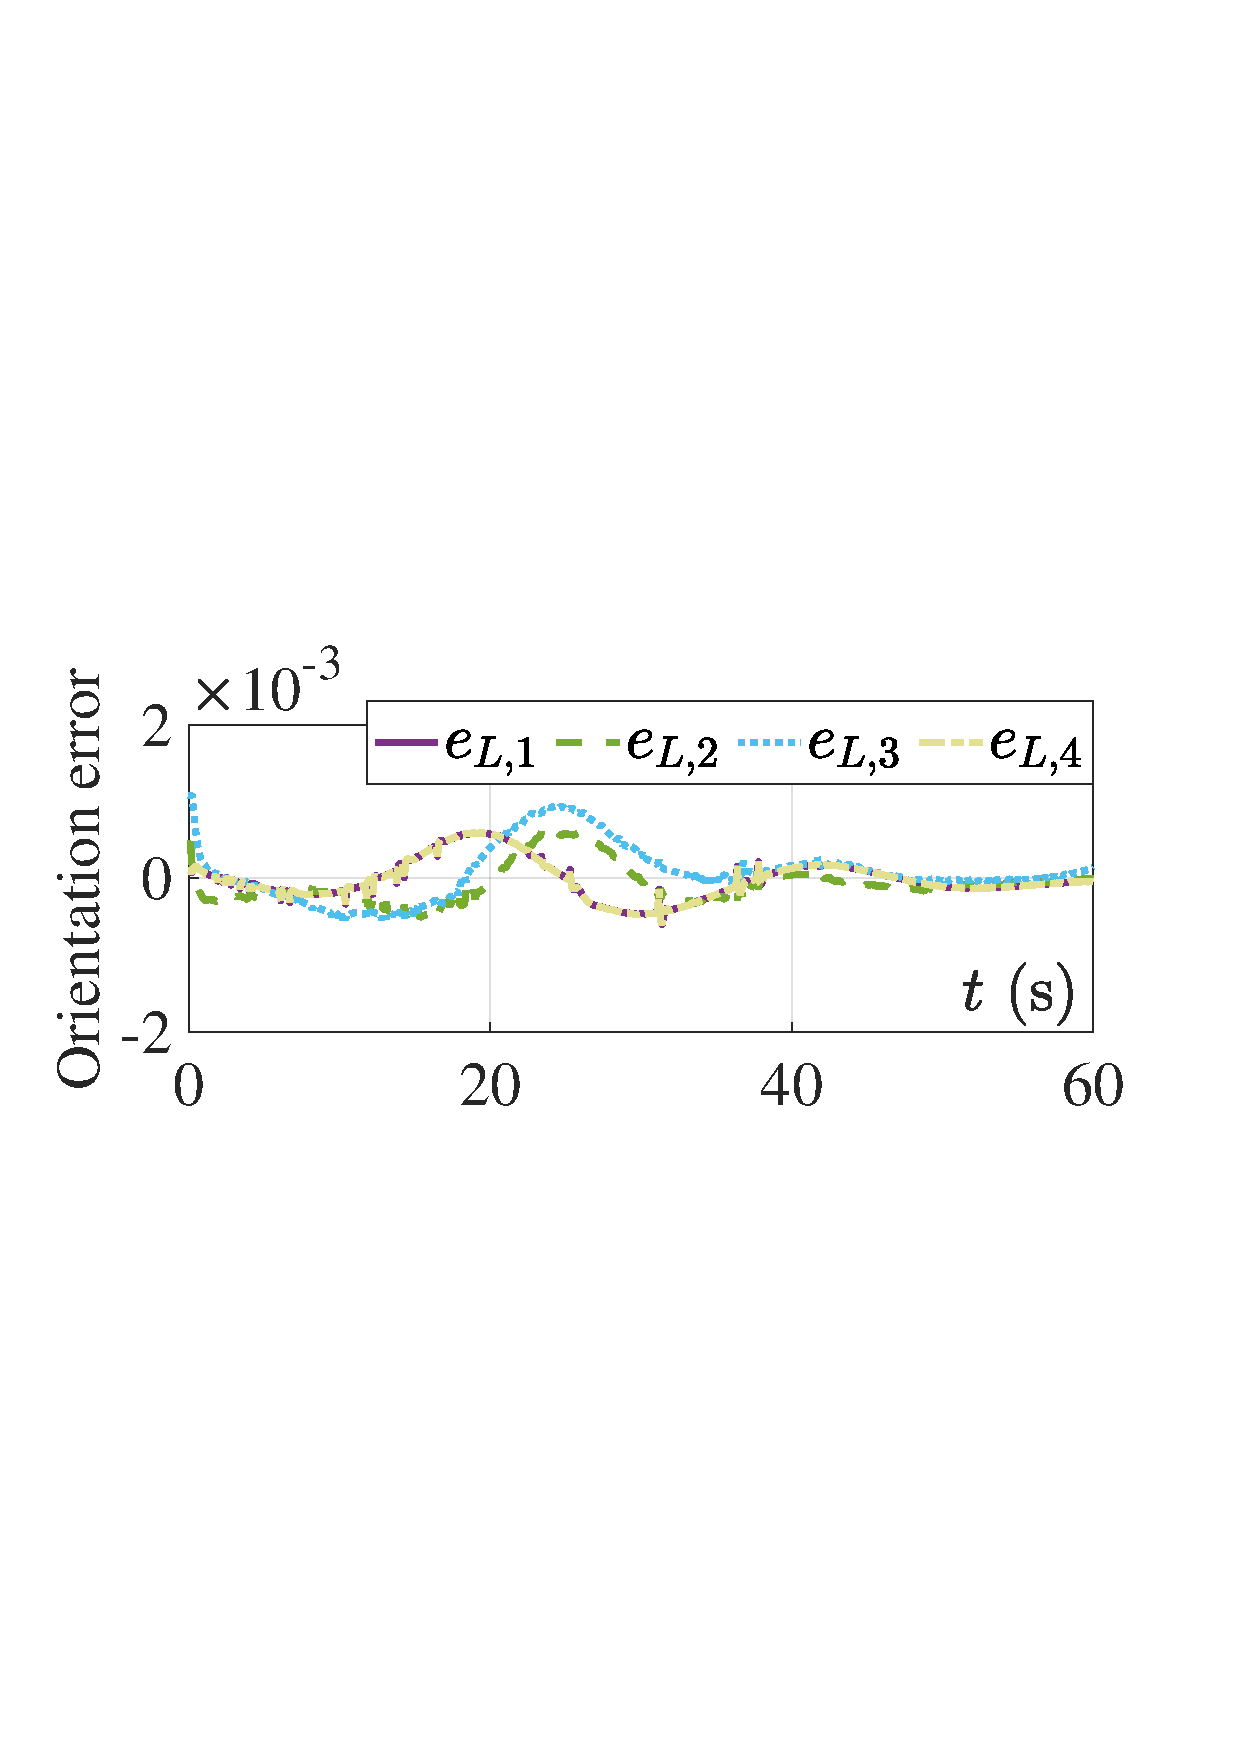
\includegraphics[width=0.45\linewidth]{figures/simulation/FIG5d_TII-24-5492.pdf}
        \label{figures:simulation:circle tracking results:d}
    }
    \hspace{0in}
    \subfigure[]{
        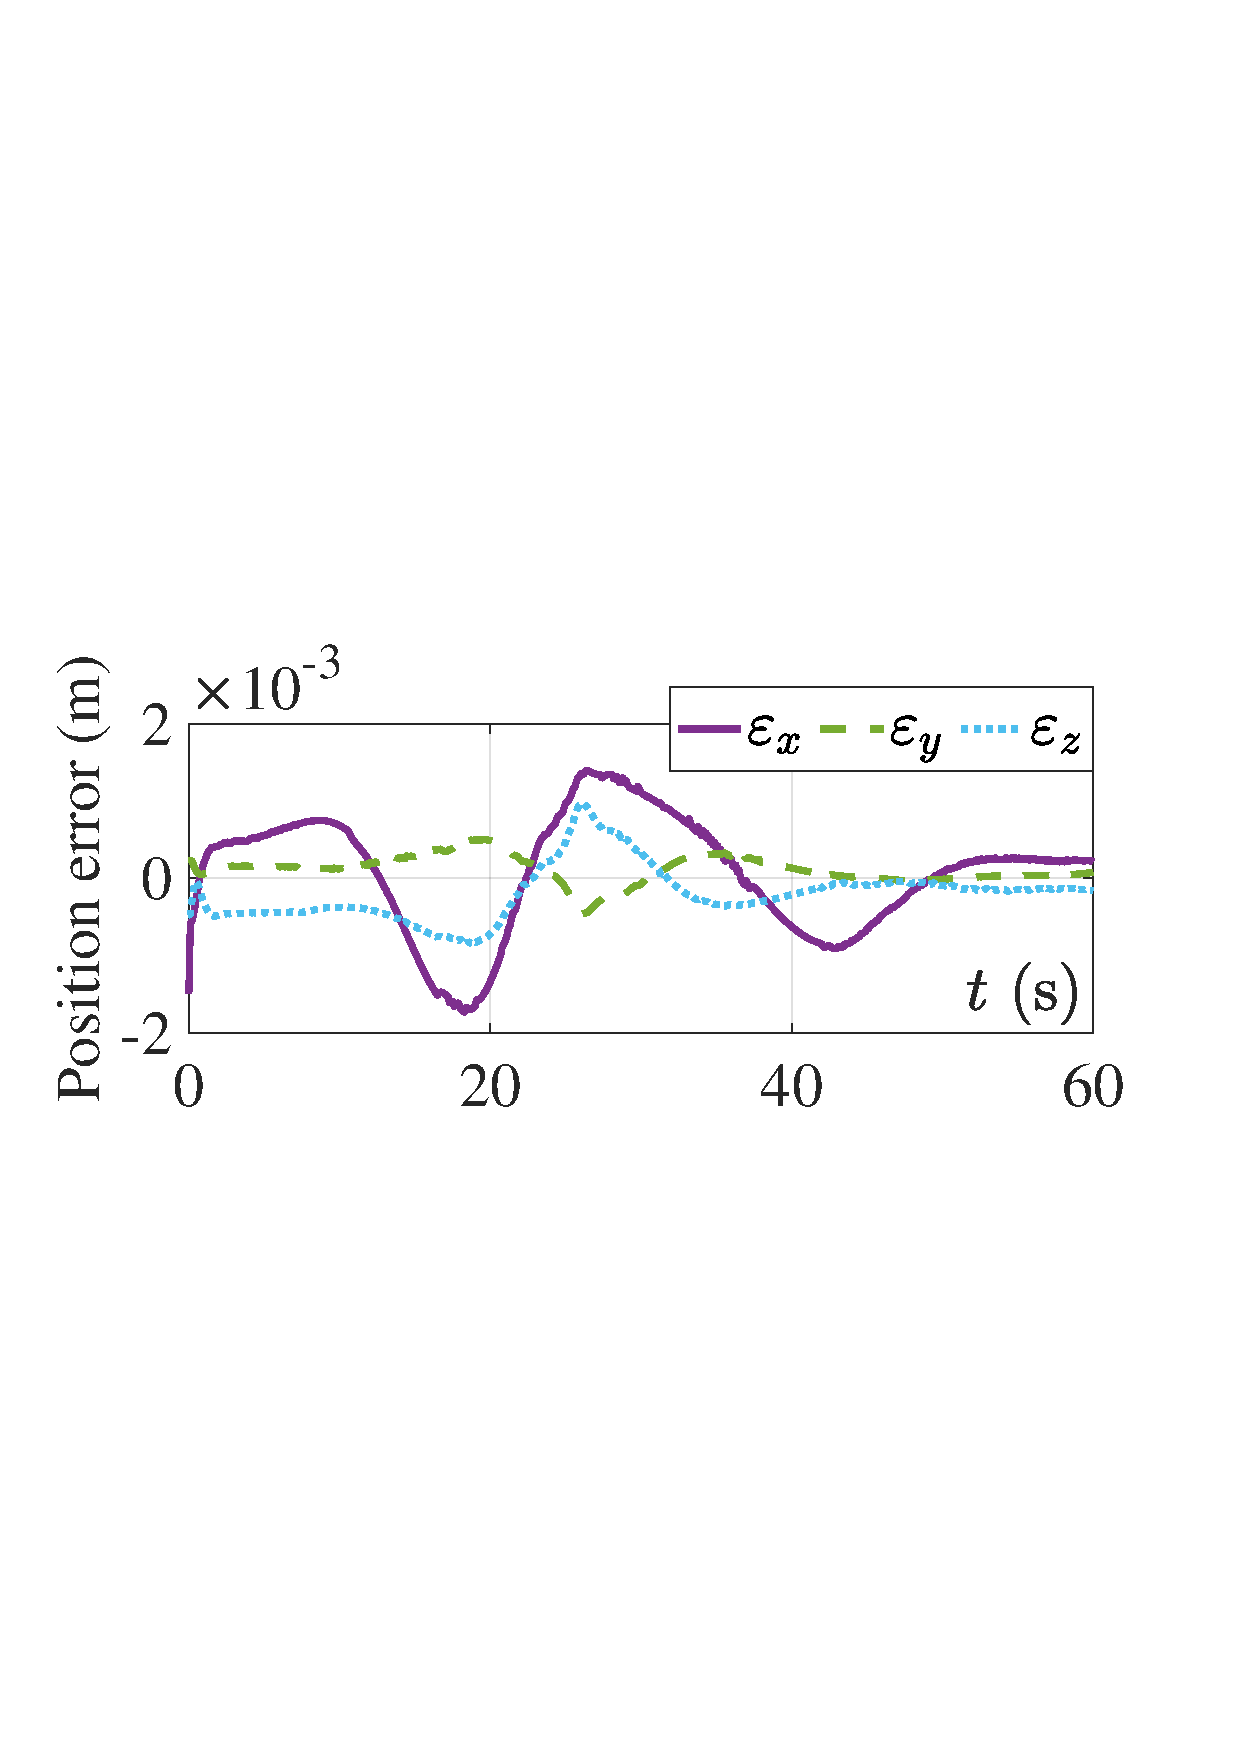
\includegraphics[width=0.45\linewidth]{figures/simulation/FIG5e_TII-24-5492.pdf}
        \label{figures:simulation:circle tracking results:e}
    }
    \hspace{0in}
    \subfigure[]{
        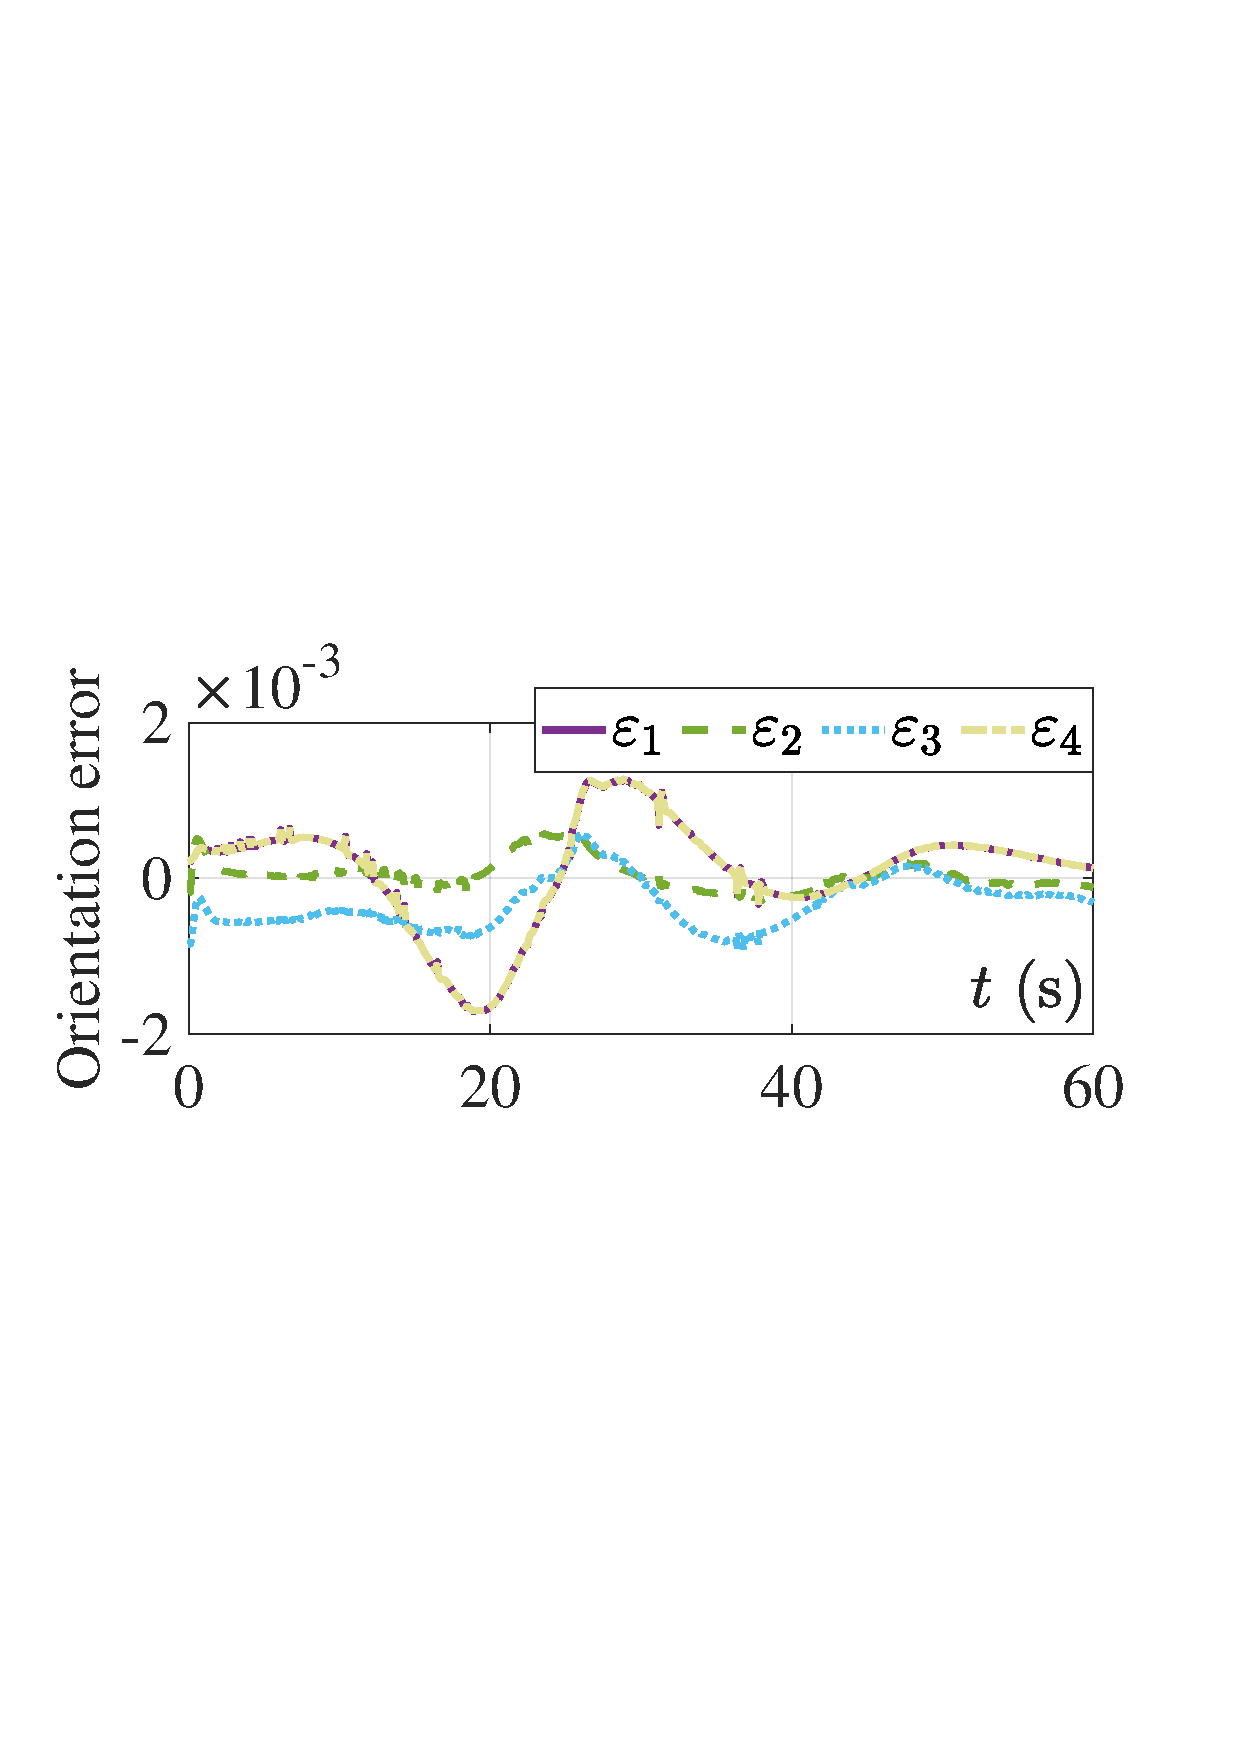
\includegraphics[width=0.45\linewidth]{figures/simulation/FIG5f_TII-24-5492.pdf}
        \label{figures:simulation:circle tracking results:f}
    }
    \caption{Tracking errors and synchronization errors of the circular trajectory tracking task in V-REP simulations. (a)-(b) Position error and orientation error of the right manipulator. (c)-(d) Position error and orientation error of the left manipulator. (e)-(f) Position and orientation synchronization errors.
    }
    \label{figures:simulation:circle tracking results}
\end{figure}

Some snapshots of the dual manipulators performing the synchronized circular trajectory tracking task in V-REP are displayed in Fig.~\ref{Fig:sim:circularPathSnapshots}(a), where the trajectories of the two modules are highlighted with magenta. It can be observed that the task has been successfully fulfilled by the dual manipulators. To further verify the effectiveness and generalizability of the proposed method, we also control dual UR5 manipulators to track more complex butterfly trajectories (as shown in Fig.~\ref{Fig:sim:circularPathSnapshots}(b)) and apply the proposed method to a coordinated transportation task (as shown in Fig.~\ref{Fig:sim:circularPathSnapshots}(c)), where the two manipulators need to coordinate to superimpose a cuboid object on another cuboid object. One can find that both the new tasks are finished successfully. More details regarding the trajectory comparison of the dual KUKA manipulators are illustrated in Fig.~\ref{figures:simulation:path comparison}. It can be seen that the actual module trajectories track the desired trajectories well. Besides, the orientations of the modules are also illustrated by blue links in Fig.~\ref{figures:simulation:path comparison}(b), which reveals that the orientations of the modules maintain unchanged during the tracking process as expected. Fig.~\ref{figures:simulation:circle tracking results} illustrates the tracking errors (i.e., $e_{R}$ and $e_{L}$) and synchronization error (i.e., $\varepsilon$) during the tracking task. The errors in the later stage of the tracking task are apparently lower than those in the earlier stage because of the continuous learning ability of cerebellar neural networks.


\begin{table}[tbp]
\centering
\caption{Evaluation for Kinematics Learning in MATLAB.}
\begin{tabular}{ccc}
\toprule
Mean Error                & Left Manipulator & Right Manipulator \\ \midrule
$M(\xi)$                     & $3.5353\times 10^{-8}$                & $3.5368\times 10^{-8}$               \\
$M(\|J-\tilde{J}\|_2)$ & 0.1523                & 0.1521                 \\ \bottomrule
\end{tabular}
\label{table:simulation:Jacobian}
\end{table}

\begin{table*}[tbp]
\centering
\caption{Property Comparison of Different Coordinated Control Methods.}
\begin{tabular}{ccccccc}
\toprule
Method  & \begin{tabular}[c]{@{}c@{}}Kinematic vs. \\ Dynamic\end{tabular} & \begin{tabular}[c]{@{}c@{}}Centralized vs.  \\ Distributed\end{tabular} & \begin{tabular}[c]{@{}c@{}}Handling  \\ synchronization  error\end{tabular} & \begin{tabular}[c]{@{}c@{}}Handling\\ secondary  tasks\end{tabular} & Robot model     & Bio-inspired control \\ \midrule
Ours    & Kinematic                                                        & Centralized                                                             & Yes                                                                         & Yes                                                                & Unknown         & Yes                  \\
Method~\cite{Chen2020} & Kinematic                                                        & Distributed                                                             & No                                                                          & No                                                                 & Known           & No                   \\
Methods~\cite{Zhang2021TNNLS,Jia2020Robotica,Zhan2024TNNLS} & Kinematic                                                        & Distributed                                                             & No                                                                          & Yes                                                                 & Known           & No                   \\
Method~\cite{Song2021} & Dynamic                                                          & Distributed                                                             & No                                                                          & No                                                                 & Known           & No                   \\
Methods~\cite{Zhai2022,Sun2002} & Dynamic                                                             & Centralized                                                             & Yes                                                                         & No                                                                 & Partially known & No                   \\ \bottomrule
\end{tabular}
\label{table:property comparison}
\end{table*}

\begin{figure}[!t]
    \centering
    \subfigure[]{
       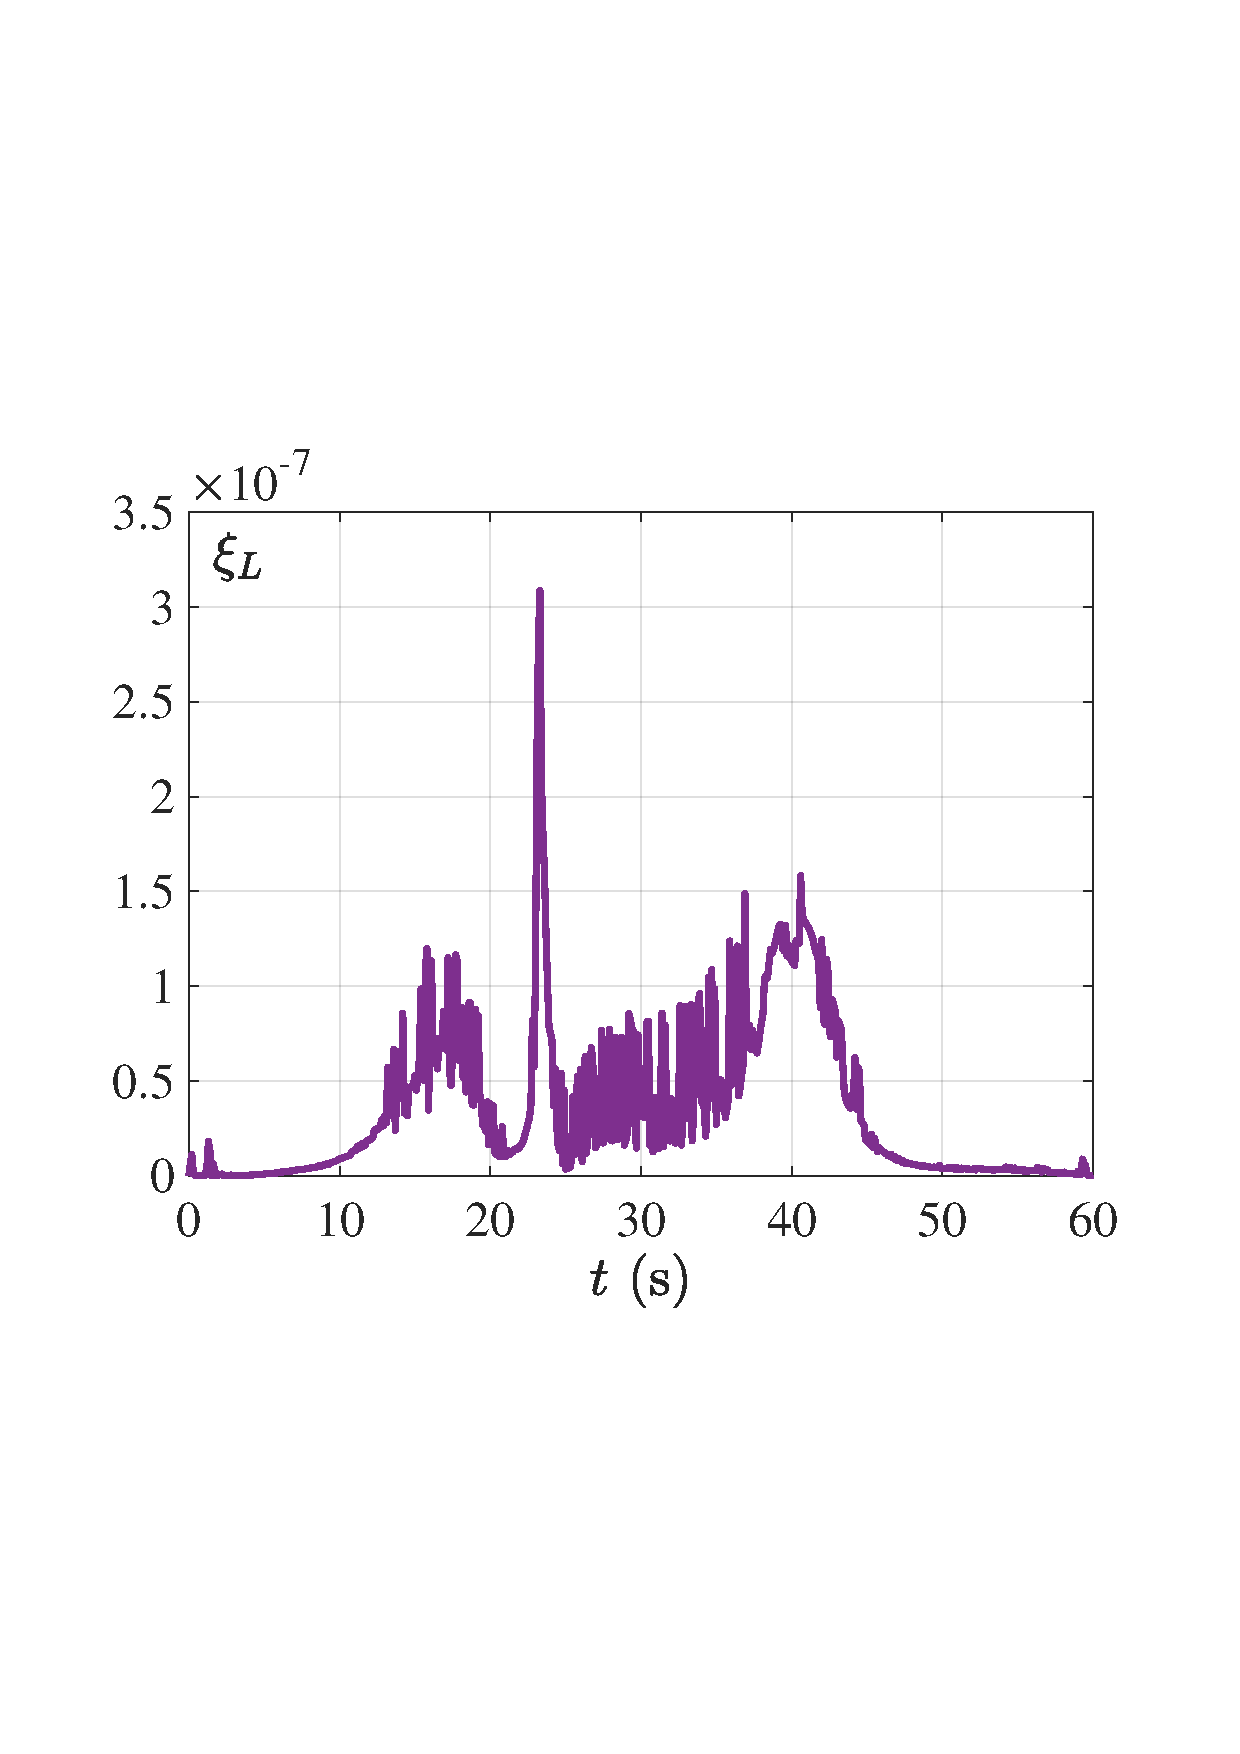
\includegraphics[width=0.44\linewidth]{figures/simulation/FIG6a_TII-24-5492.pdf}
        \label{figures:simulation:Jacobian:a}
    }
    \hfill
    \subfigure[]{
        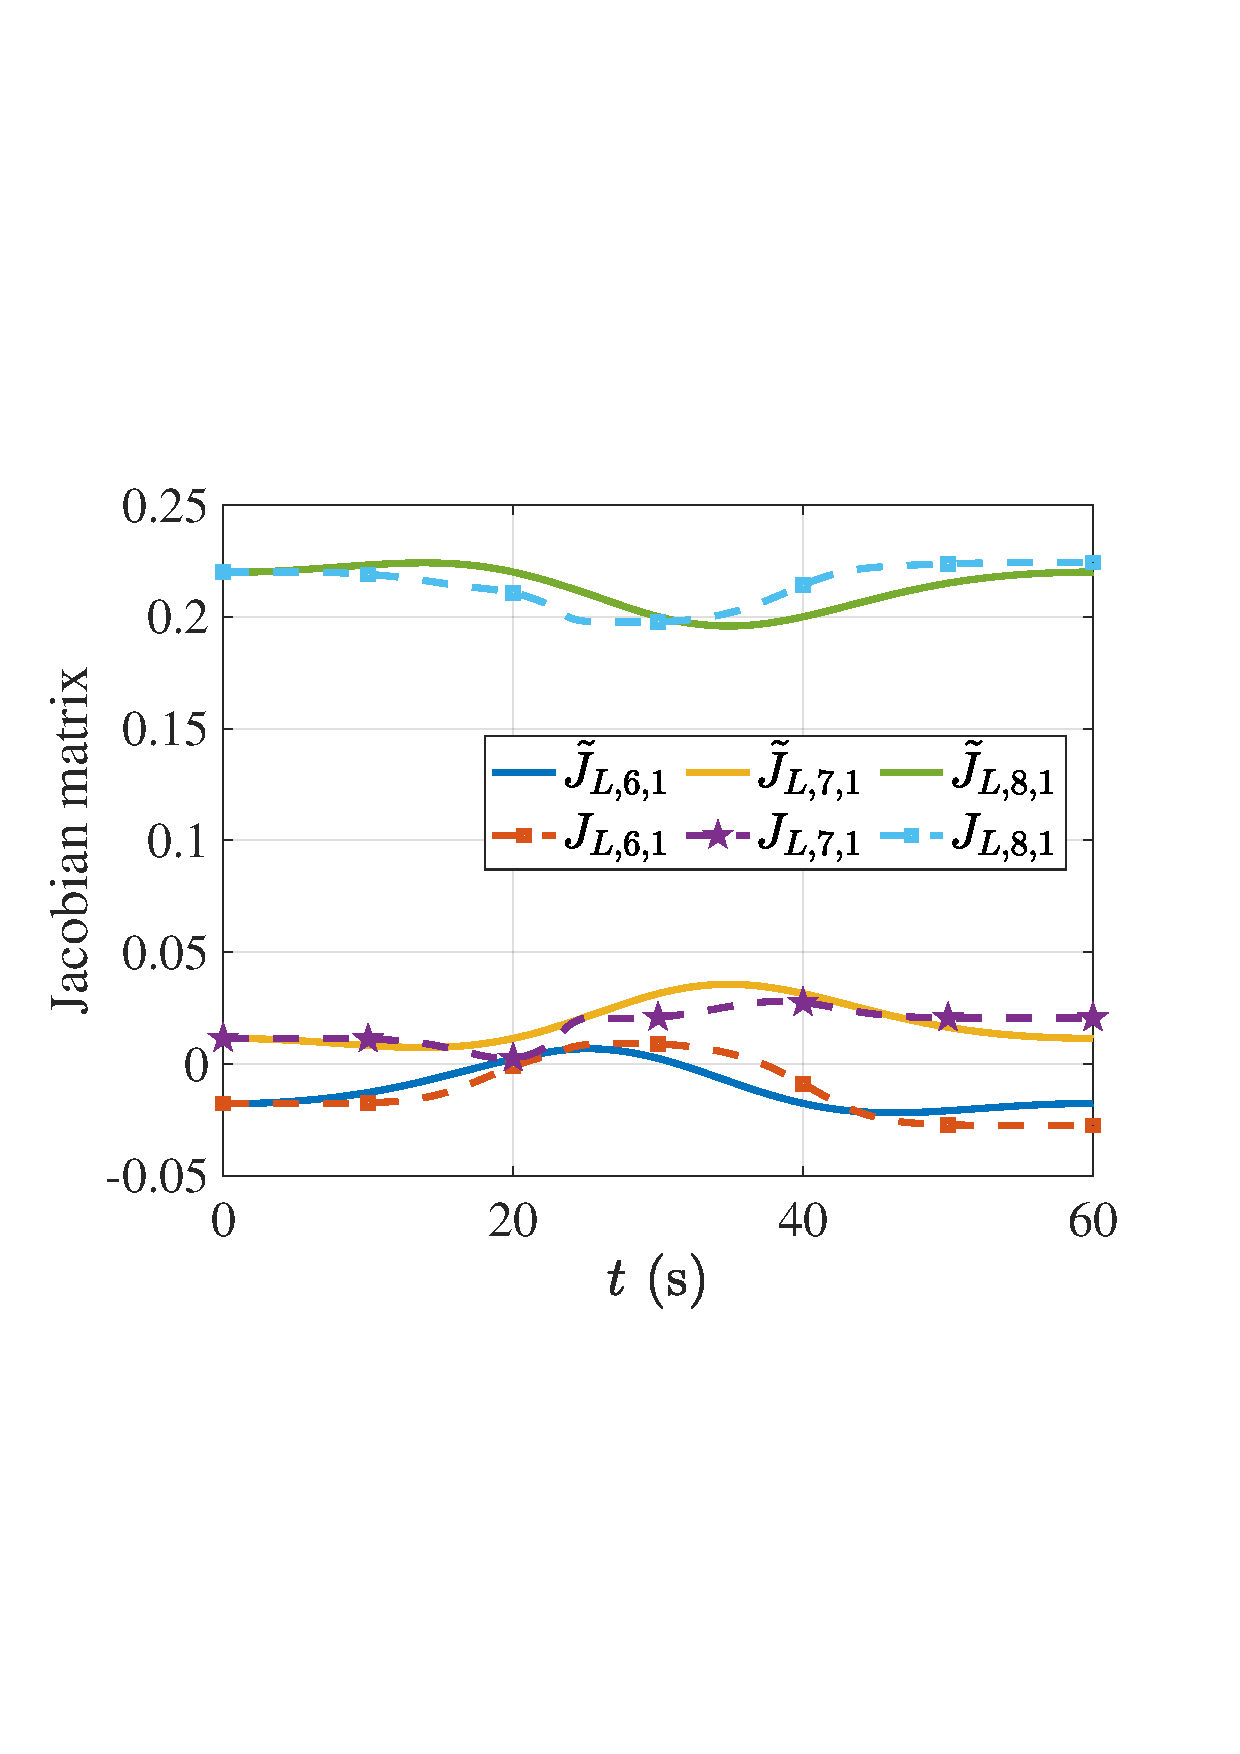
\includegraphics[width=0.47\linewidth]{figures/simulation/FIG6b_TII-24-5492.pdf}
        \label{figures:simulation:Jacobian:bs}
    }
    \caption{Simulation results of kinematics learning for the left manipulator. (a) Profile of the norm-based energy function $\xi_L$. (b) Comparison between the elements of the analytical Jacobian matrix $J_L$ and the elements of the learned Jacobian matrix $\tilde{J}_L$.
    }
    \label{figures:simulation:Jacobian}
\end{figure}


To verify the effectiveness of the proposed kinematics learning method, we utilize the robotics system toolbox in MATLAB to simulate two robots and control them with our control system. The toolbox enables us to calculate the analytical value of Jacobian matrices  and verify the accuracy of learned Jacobian matrices. As illustrated in Table~\ref{table:simulation:Jacobian}, the mean values of the energy function $\xi$ defined for kinematics learning are $3.5353\times 10^{-8}$ and $3.5368\times 10^{-8}$, respectively. The mean values of Jacobian estimation error $\|J-\tilde{J}\|_2$ of the robots are $0.1523$ and $0.1521$, respectively. As an example, profiles of the norm-based energy function and the comparison between some elements of the analytical Jacobian matrix and some elements of the learned Jacobian matrix of the left manipulator are depicted in Fig.~\ref{figures:simulation:Jacobian}, which reveals the effectiveness of the proposed kinematics learning method.


\subsection{Comparison}

\begin{figure}[!t]
    \centering
    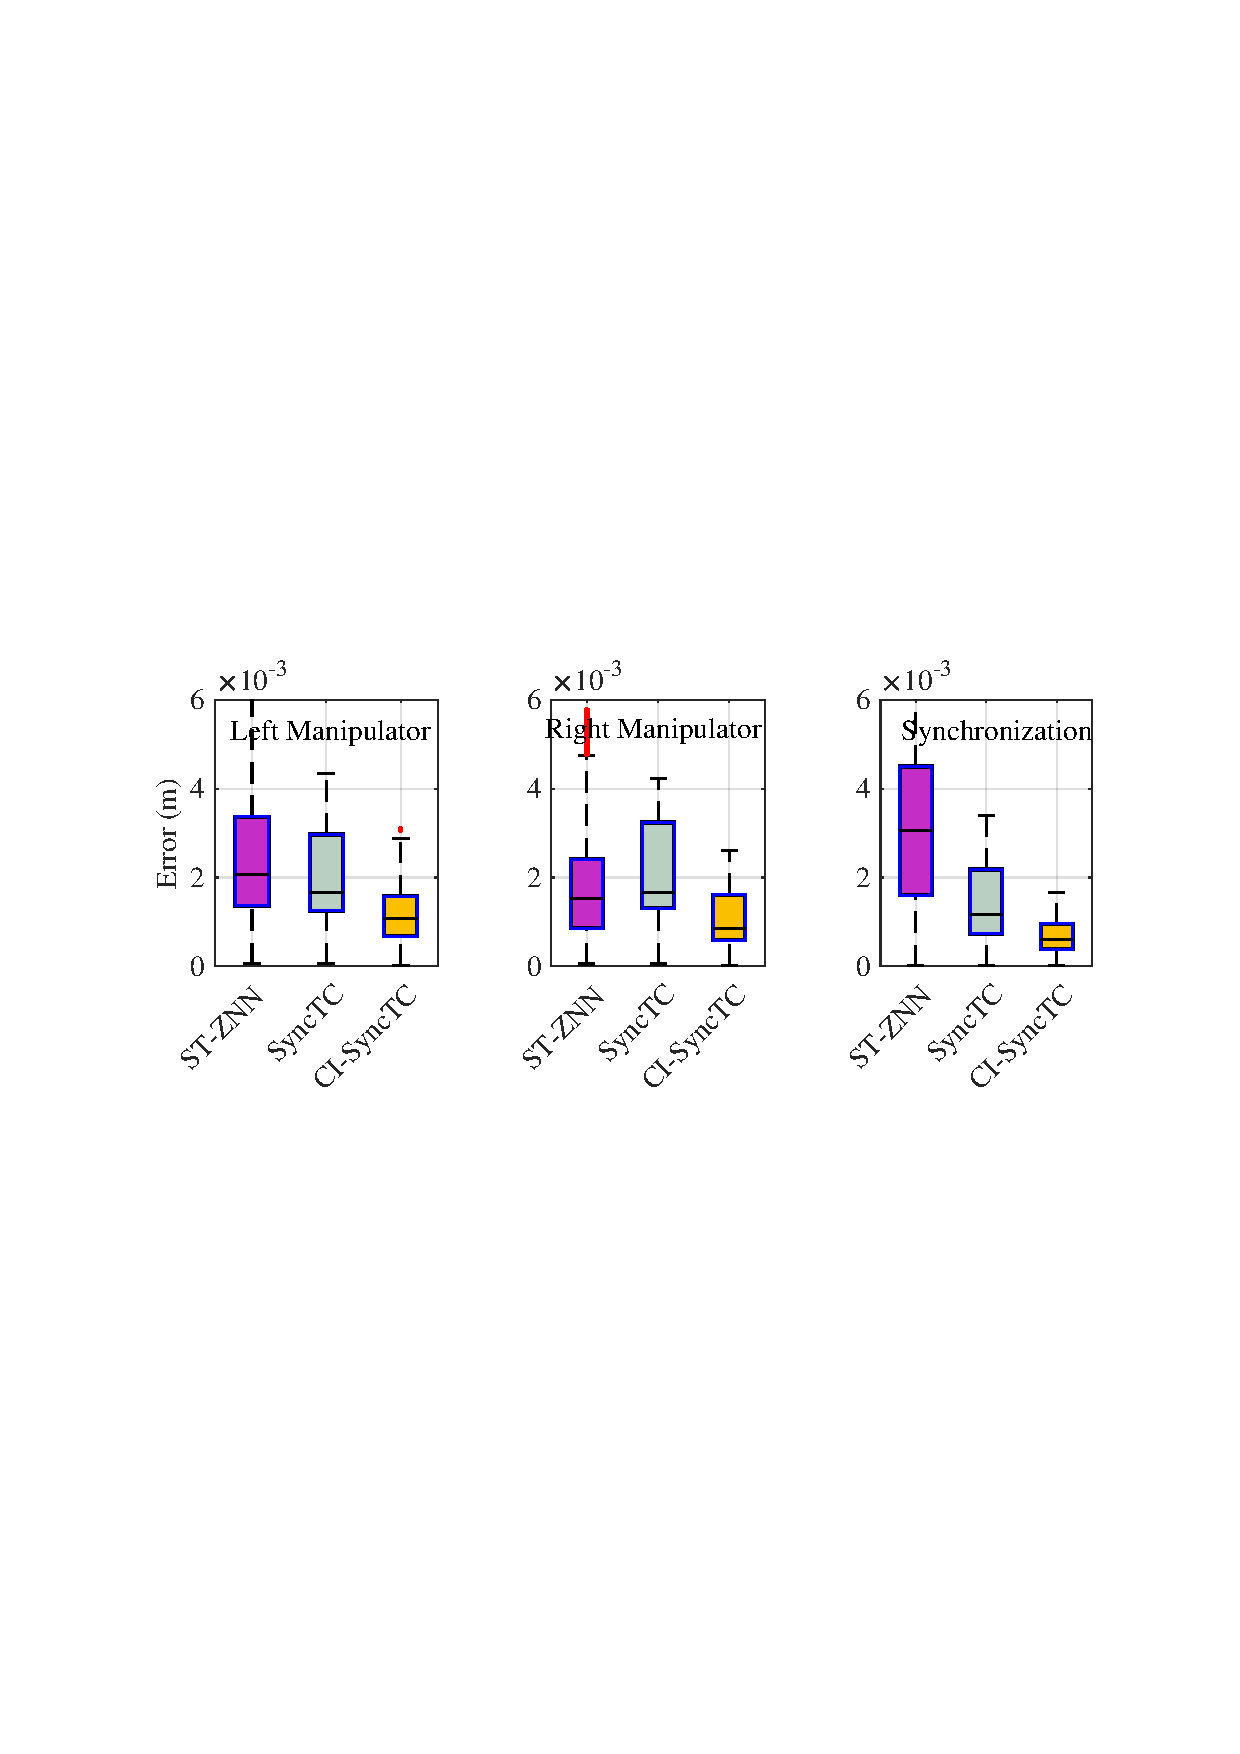
\includegraphics[width=1\linewidth]{figures/simulation/FIG7_TII-24-5492.pdf}
    \caption{Box-plot of position tracking errors and synchronization errors associated with different control methods.
    }
    \label{Fig:sim:comparison}
\end{figure}

\begin{table}[!tbp]
\centering
\caption{Quantitative Comparison of Different Control Methods.}
\tabcolsep=5pt
\begin{tabular}{clll}
\toprule
Method                                       & $M(e_L)$ & $M(e_R)$ & $M(\varepsilon)$ \\ \midrule
ST-ZNN~\cite{Chen2020} & 2.7 mm   & 1.9 mm   & 3.1 mm   \\
SyncTC                                       & 2.1 mm   & 2.1 mm   & 1.5 mm   \\
CI-SyncTC                                    & 1.1 mm ($\downarrow$ 47\%)   & 1.1 mm ($\downarrow 47$\%)  & 0.8 mm ($\downarrow 46$\%)  \\ \bottomrule
\end{tabular}
\label{table:method comparison}
\end{table}

In this part, we compare the proposed method with existing coordinated control methods both qualitatively and quantitatively. To begin with, as shown in Table~\ref{table:property comparison}, we compare the properties of different methods. Existing control methods include kinematic control methods and dynamic control methods, and this work belongs to the former. Unlike existing distributed kinematic control methods, our centralized method can handle synchronization error, thereby achieving better coordination performance. More importantly, our method is the first bio-inspired coordinated control method for robot manipulators with unknown kinematic models. These qualitative comparisons reveal the novelty of our method. Then, simulations on the synchronized control of dual KUKA manipulators are carried out for the quantitative comparison purpose. Specifically, we take the super twisting zeroing neural network (ST-ZNN) method~\cite{Chen2020} as a comparison for the kinematic bimanual coordination problem. To reveal the learning ability of the cerebellar neural network, we also take our proposed synchronized tracking control (SyncTC) method~\eqref{eq:QP} as a comparison, which is obtained by removing cerebellar neural networks in our CI-SyncTC method. Intuitive comparison results are illustrated in Fig.~\ref{Fig:sim:comparison}, including the position tracking errors and the synchronization errors associated with different control methods. For a quantitative comparison, the mean position tracking errors and mean position synchronization errors are summarized in Table~\ref{table:method comparison}, where $M$ denotes mean position error. The results indicate that our proposed SyncTC method can achieve a similar level of mean tracking errors (2.1 mm for both the manipulators) compared to the ST-ZNN method (2.7 mm for the left manipulator and 1.9 mm for the right manipulator). However, the ST-ZNN method has achieved much larger synchronization error (3.1 mm) than our SyncTC method (1.5 mm). By incorporating cerebellar neural networks, our CI-SyncTC method has achieved lower tracking errors (reduced by 47\%) and synchronization error (reduced by 46\%) than the SyncTC method.


\begin{figure}[!t]
    \centering
    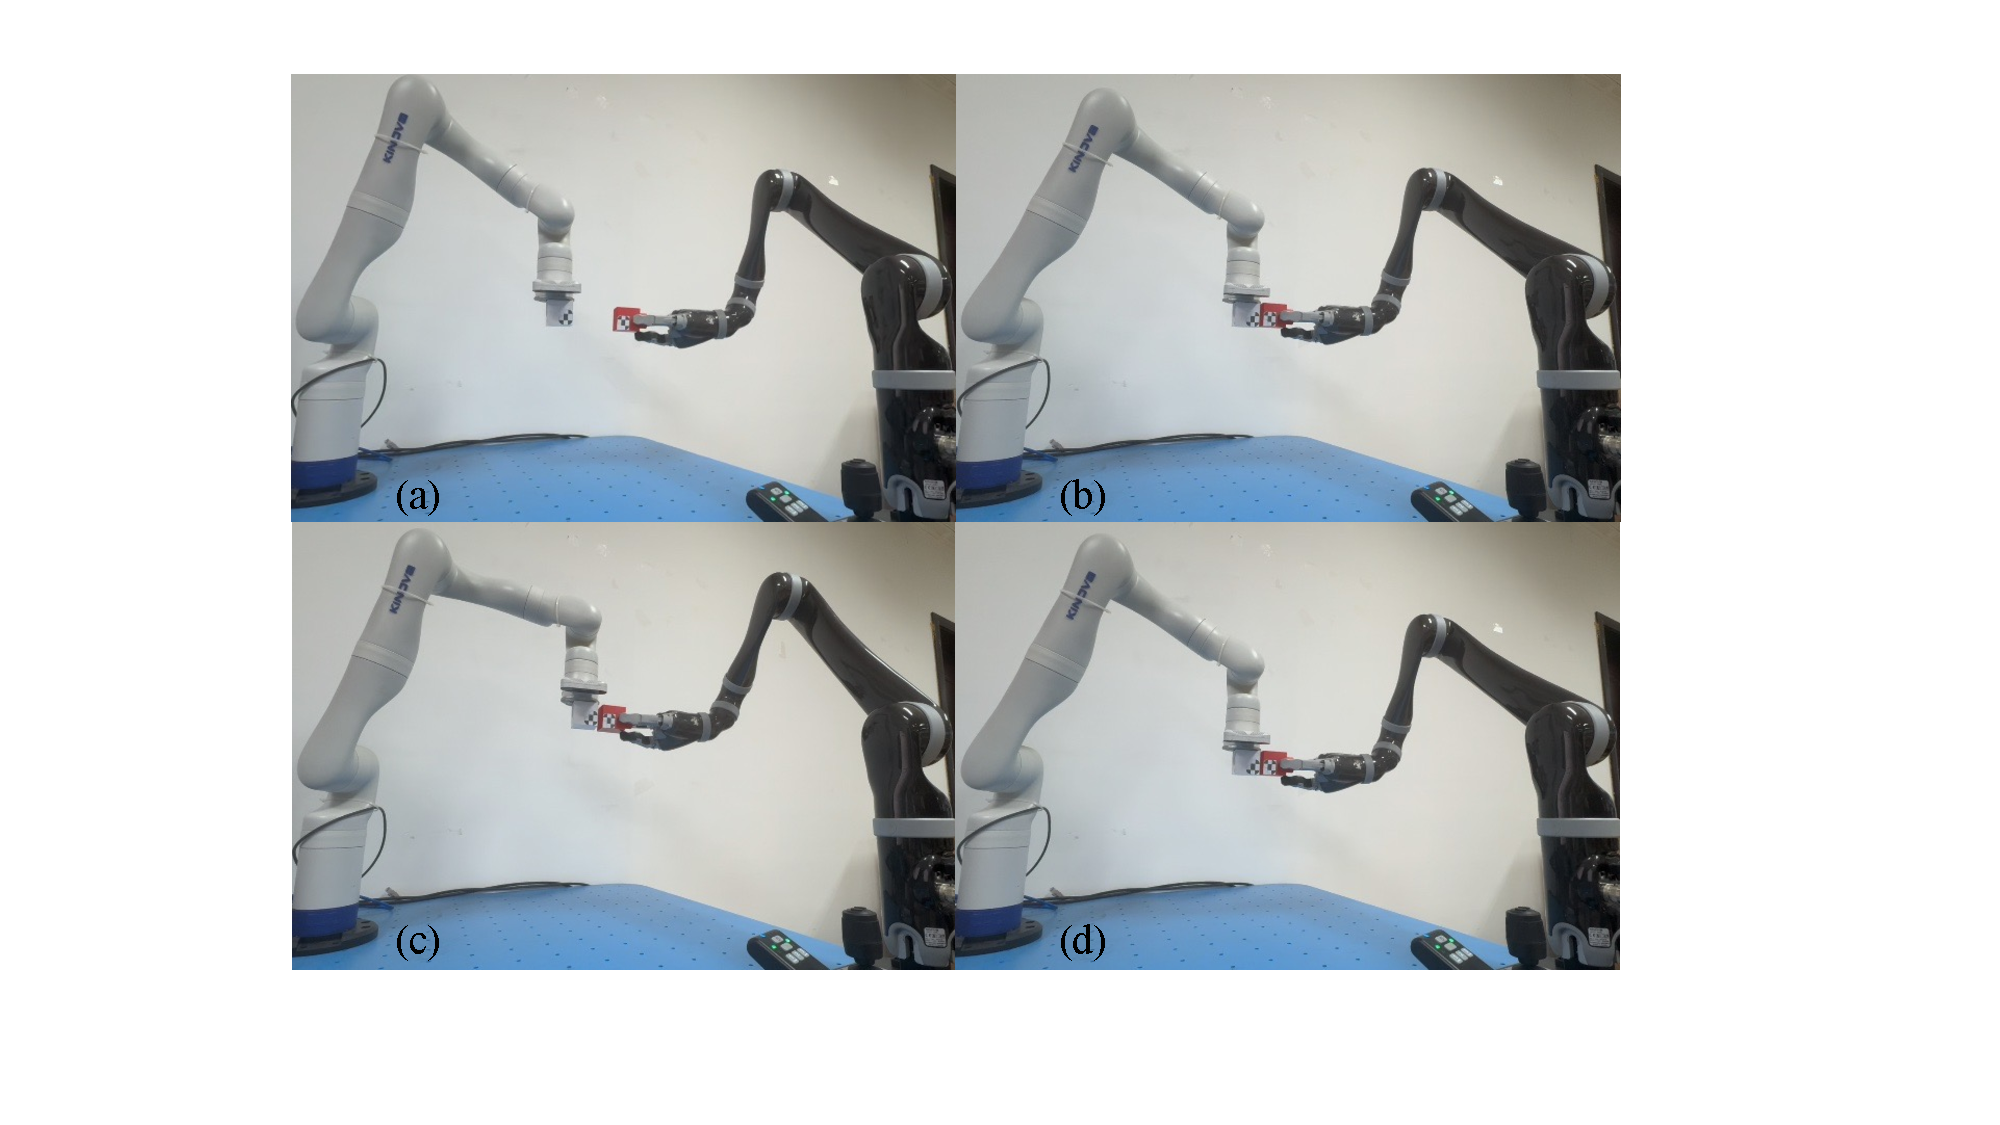
\includegraphics[width=0.9\linewidth]{figures/experiment/FIG8_TII-24-5492.pdf}
    \caption{Experiment snapshots of the synchronized trajectory tracking task. (a) Initial configuration. (b) Dual manipulators align the two modules. (c) Dual manipulators perform the synchronized tracking task. (d) Dual manipulators have finished the coordination task.
    }
    \label{Fig:exp:snapshots}
\end{figure}


\subsection{Experiment}


In this part, physical experiments are conducted to verify the effectiveness of our method. The experiment setup is shown in Fig.~\ref{Fig:exp:snapshots}, including KINOVA Jaco Gen-3 (7 DOF) and Gen-2 (6 DOF) manipulators. Likewise, our task is to control the dual manipulators to align the white module and the red module, and move them along circular trajectories synchronously while maintaining the module orientation unchanged. The synchronization coefficient is set as $k_s= 0.1$. The convergence coefficient for the kinematics learning is set as $\lambda = 0.5$. The convergence rate of the zeroing neurodynamic model is chosen as $\gamma = 0.8$. For the cerebellar neural network, the number of GCs is $400$, the leakage rate is $k_l = 0.6$, the speed of the dynamics is $k_g = 0.5$, and the learning rate $\eta$ is set to $1\times 10^{-4}$. 

\begin{remark}
When estimating the Jacobian matrix, the end-effector velocity is obtained by differentiating pose. As for the joint velocity, we directly use the joint velocity generated by our control system instead of that measured by sensors, assuming that the robot can track the joint velocity command well. In our experiments, the Micron Tracker H3-60 sensor is adopted to measure the pose information, which officially claims an accuracy of 0.2 mm in terms of position. We adopt a low-pass filter to process pose information~\cite{Yang2020TIE}, which can deal with sensor noises and provide velocity information.
\end{remark}

\begin{figure}[!t]
    \centering
    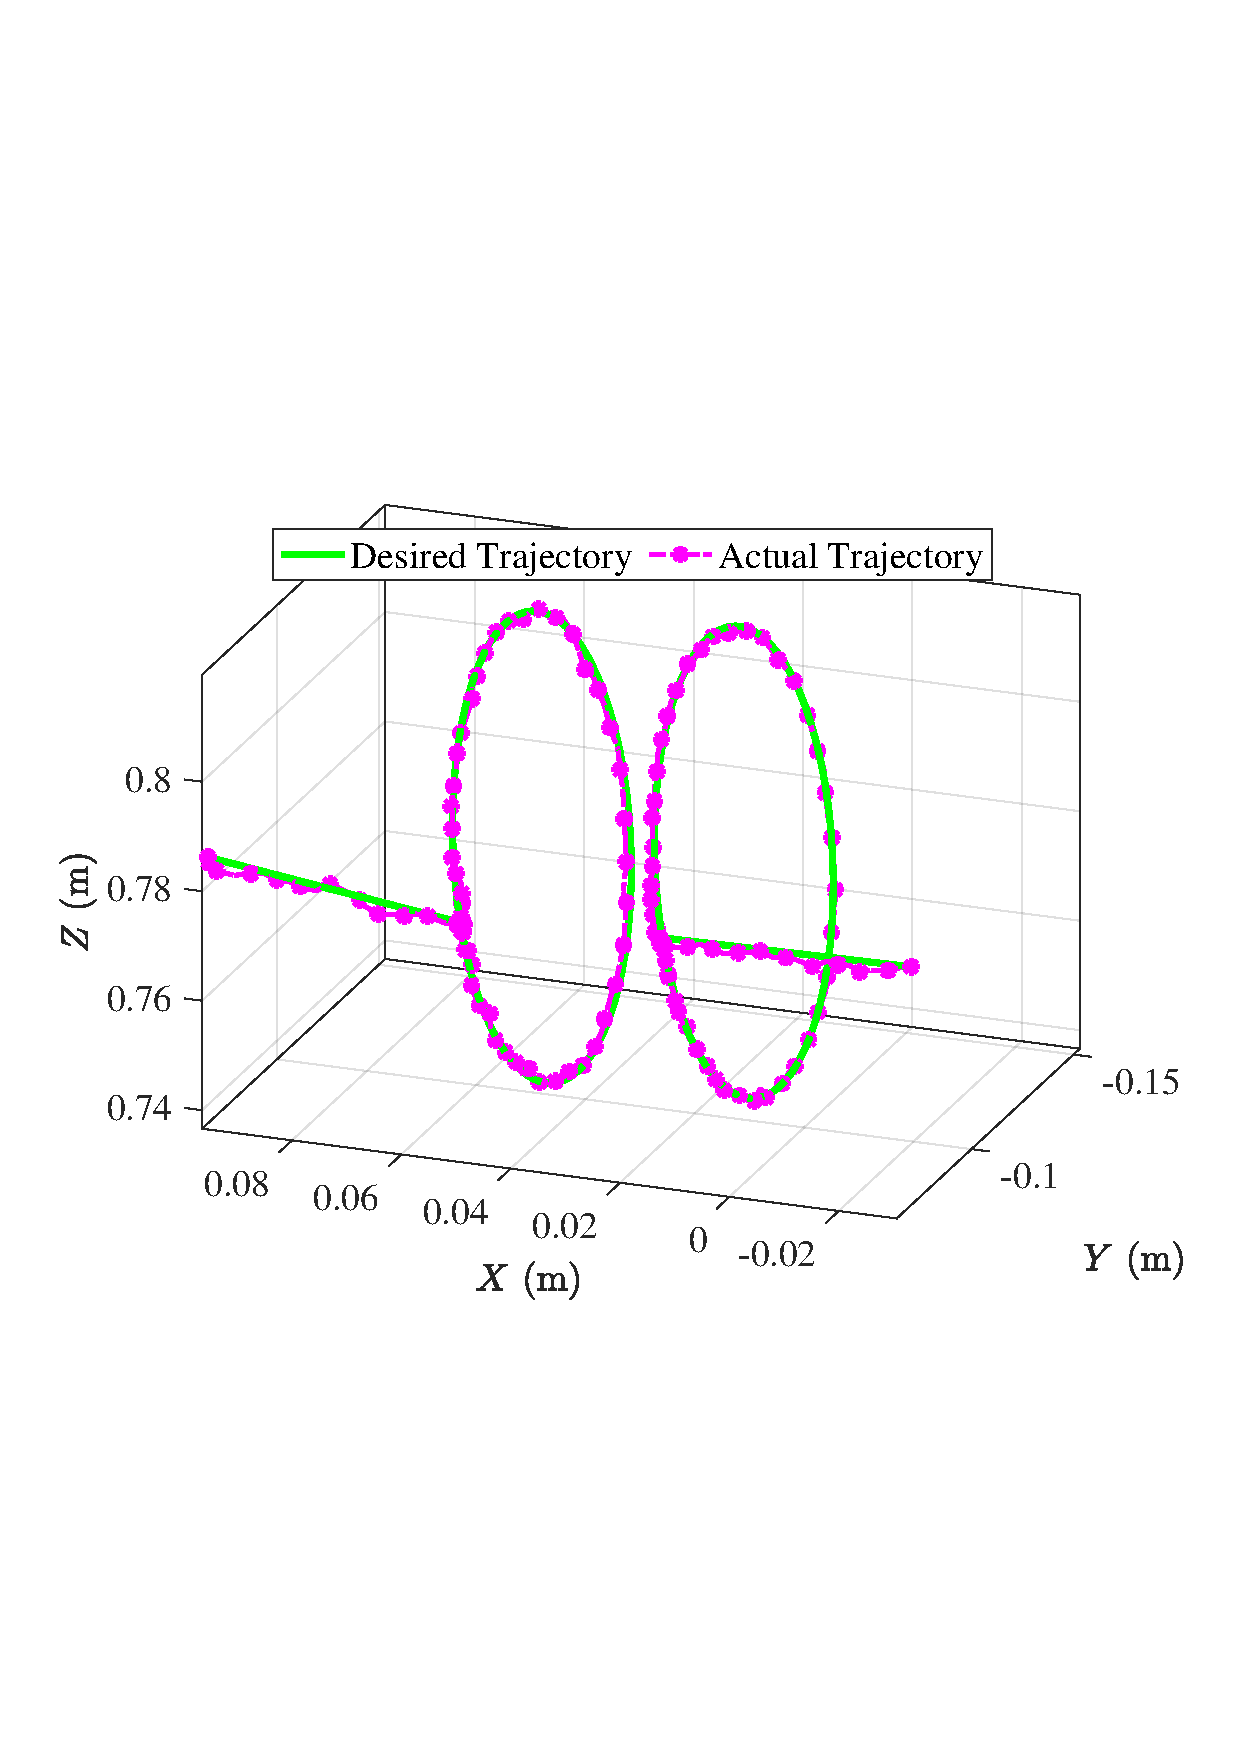
\includegraphics[width=0.7\linewidth]{figures/experiment/FIG9_TII-24-5492.pdf}
    \caption{Profiles of the desired trajectories and the actual trajectories of manipulators synthesized by our CI-SyncTC method in physical experiments.
    }
    \label{figures:experiment:path comparison}
\end{figure}



Some snapshots of the physical manipulators performing the synchronized tracking task are depicted in Fig.~\ref{Fig:exp:snapshots}, and the trajectory comparison is illustrated Fig.~\ref{figures:experiment:path comparison}. We can find that the actual module trajectories track the desired trajectories well. Besides, the orientations of the modules maintain unchanged during the tracking process as expected. Specifically, the mean position tracking errors of the dual manipulators are 1.0 mm and 1.5 mm respectively, and the mean position synchronization error is 2.0 mm. We also compare our CI-SyncTC method with the SyncTC method and the ST-ZNN method in the experiment. Intuitive comparison results are illustrated in Fig.~\ref{Fig:experiment:comparison}, including position tracking errors and synchronization errors associated with different control methods. Similar to simulation results, the ST-ZNN method achieved much larger error on the left manipulator, although the error on the right manipulator is comparable to our CI-SyncTC method. Besides, the synchronization error of the ST-ZNN method is also larger than our methods because it cannot handle synchronization error. For a quantitative comparison, the mean position tracking errors and mean position synchronization errors are summarized in Table~\ref{table:exp:method comparison}. We can find that, compared to the SyncTC method, the mean position tracking errors of the dual manipulators are reduced by 23\% and 25\% respectively, and the mean position synchronization error is reduced by 40\% through cerebellar neural networks. Compared with the simulation part, the percentage of error reduction in the experiment is smaller because we reduced the value of learning rate to ensure stability. In summary, these experiment results have confirmed the effectiveness of our control scheme for bimanual synchronized tracking control of robotic manipulators and the ability of the cerebellar neural network in reducing tracking error and synchronization error through learning. Finally, to verify the generalizability of the proposed method across different platforms, as shown in Fig.~\ref{Fig:experiment:franka}, we replace the Jaco Gen-3 manipulator with a Franka Emika Panda manipulator and control the dual manipulators to fulfill a coordinated transportation task. One can find that the task is also fulfilled successfully. It is worth pointing out that we do not need to know the model or parameters of robots when applying our method to different robots due to its model-free nature.

\begin{figure}[!t]
    \centering
    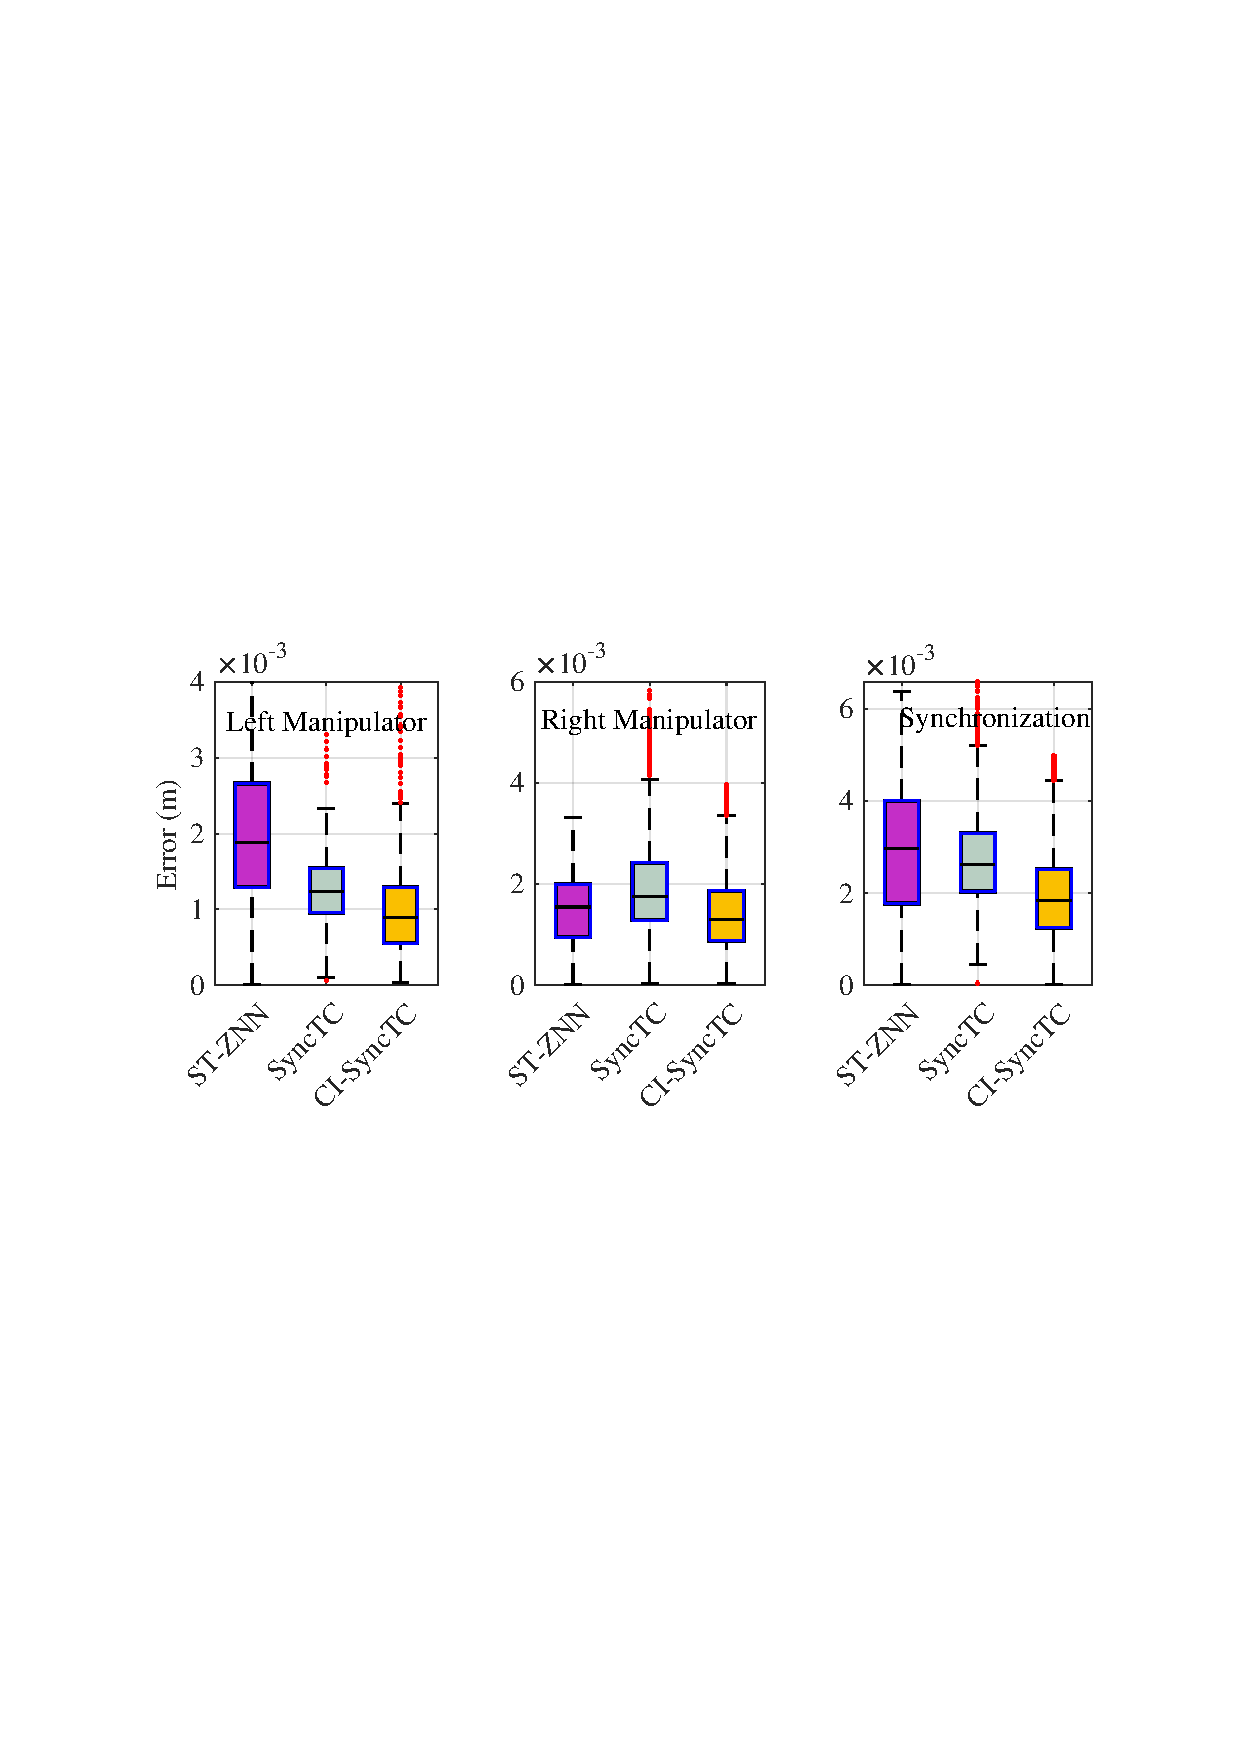
\includegraphics[width=1\linewidth]{figures/experiment/FIG10_TII-24-5492.pdf}
    \caption{Box-plot of position tracking errors and synchronization errors associated with different control methods in physical experiments.
    }
    \label{Fig:experiment:comparison}
\end{figure}

\begin{table}[!tbp]
\centering
\caption{Quantitative Method Comparison in Experiments.}
\begin{tabular}{clll}
\toprule
Method                                       & $M(e_L)$ & $M(e_R)$ & $M(\varepsilon)$ \\ \midrule
ST-ZNN~\cite{Chen2020}                                       & 2.2 mm   & 1.7 mm   & 3.4 mm   \\
SyncTC                                       & 1.3 mm   & 2.0 mm   & 2.8 mm   \\
CI-SyncTC                                    & 1.0 mm ($\downarrow$ 23\%)   & 1.5 mm ($\downarrow$ 25\%)  & 2.0 mm ($\downarrow$ 40\%)  \\ \bottomrule
\end{tabular}
\label{table:exp:method comparison}

\end{table}
\begin{figure}[!t]
    \centering
    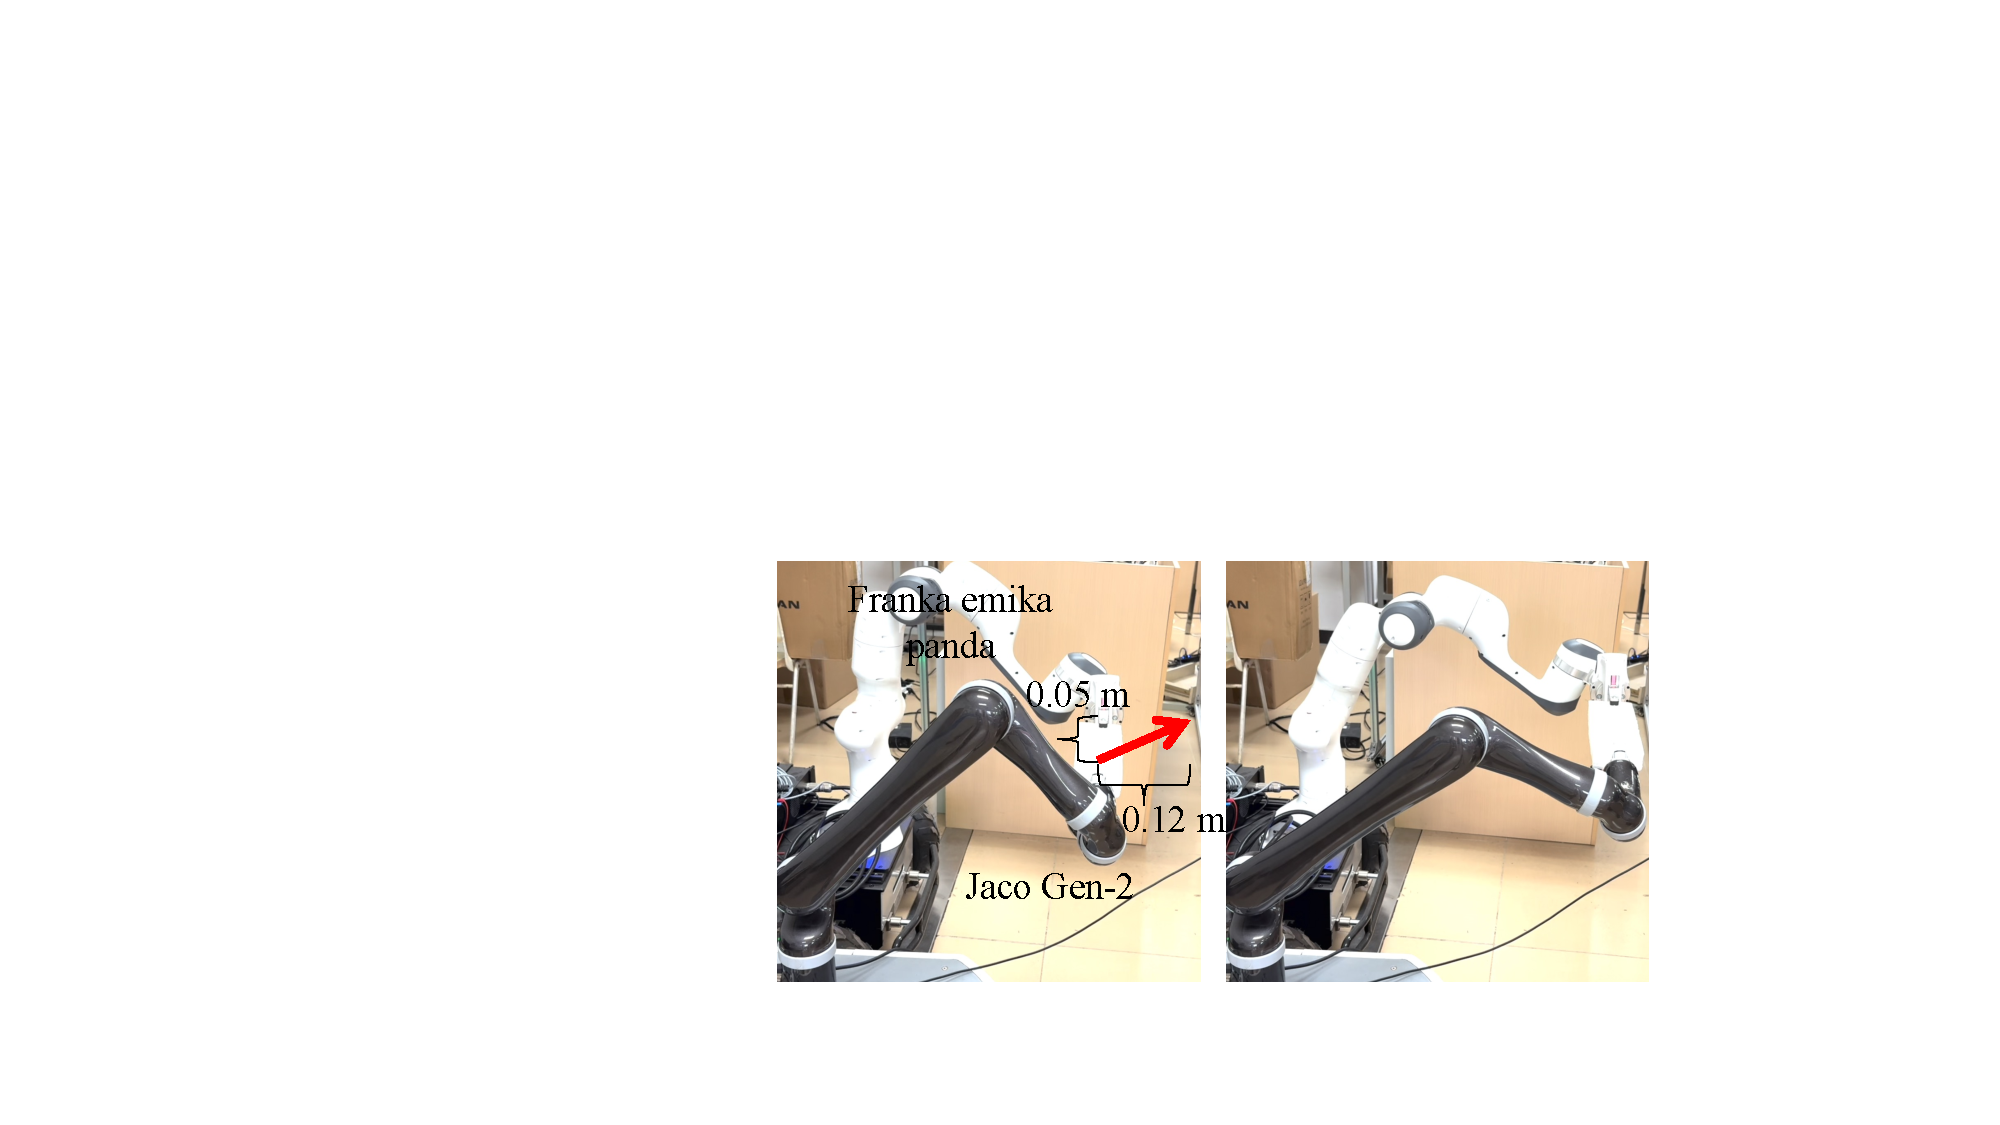
\includegraphics[width=0.9\linewidth]{figures/experiment/FIG11_TII-24-5492.pdf}
    \caption{Coordinated transportation of a Jaco Gen-2 manipulator and a Franka Emika Panda manipulator.
    }
    \label{Fig:experiment:franka}
\end{figure}

\section{Conclusion} \label{section:conclustion}

In this paper, the bimanual synchronized tracking control of dual robotic manipulators with uncertain kinematics has been studied. First, the gradient neurodynamic method can estimate the unknown kinematics of robot manipulators, which is essential to the kinematic control. Then, the synchronized tracking control problem has been solved by utilizing zeroing neurodynamics and quadratic programming. Furthermore, a cerebellar neural network has been proposed to endow the control system with continuous learning ability. Finally, the simulative and experimental results have shown that the proposed hybrid neurodynamic scheme can achieve the synchronized tracking control of dual robotic manipulators successfully. Additionally, as a result of the learning ability of the cerebellar neural network, the tracking errors of the manipulators and the synchronization error can be reduced. It is notable that the whole control system requires no pre-training phase and can learn entirely online, which means the cerebellar learning and tracking task are performed simultaneously. Furthermore, the proposed scheme can quickly adapt to different types of manipulators without special adjustment due to its model-free nature, demonstrating its adaptability.

\bibliographystyle{ieeetr}
\bibliography{reference}

\begin{IEEEbiography}[{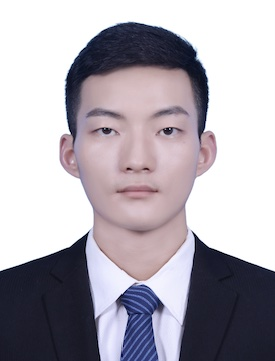
\includegraphics[width=1in,height=1.25in,clip,keepaspectratio]{figures/Peng_Yu.jpg}}]
   {Peng Yu} received the B.E. and M.E. degrees in software engineering in 2019 and 2021, respectively, from Sun Yat-Sen University, Guangzhou, China, where he is currently working toward the Ph.D. degree in computer science and technology with the School of Computer Science and Engineering. His current research interests include soft robots, industrial robots, and intelligent control.
\end{IEEEbiography}
\begin{IEEEbiography}[{
\includegraphics[width=1in,height=1.25in,clip,keepaspectratio]{figures/Ning_Tan.jpg}}]
   {Ning Tan} received the Ph.D. degree in automation from the Department of Automatic Control and Micro-Mechatronic Systems, Université de Franche-Comté/Franche-Comté Electronics Mechanics Thermal Science and Optics–Sciences and Technologies Institute, Besançon, France, in 2014.

   He is currently an associate professor with Sun Yat-sen University, Guangzhou, China. From 2014 to 2018, he held a post-doctoral position and research fellow position at the Singapore University of Technology and Design and National University of Singapore, Singapore. His research interests include soft robotics, bioinspired design, modular and reconfigurable mechanisms, and micronano robotics.
\end{IEEEbiography}
\begin{IEEEbiography}[{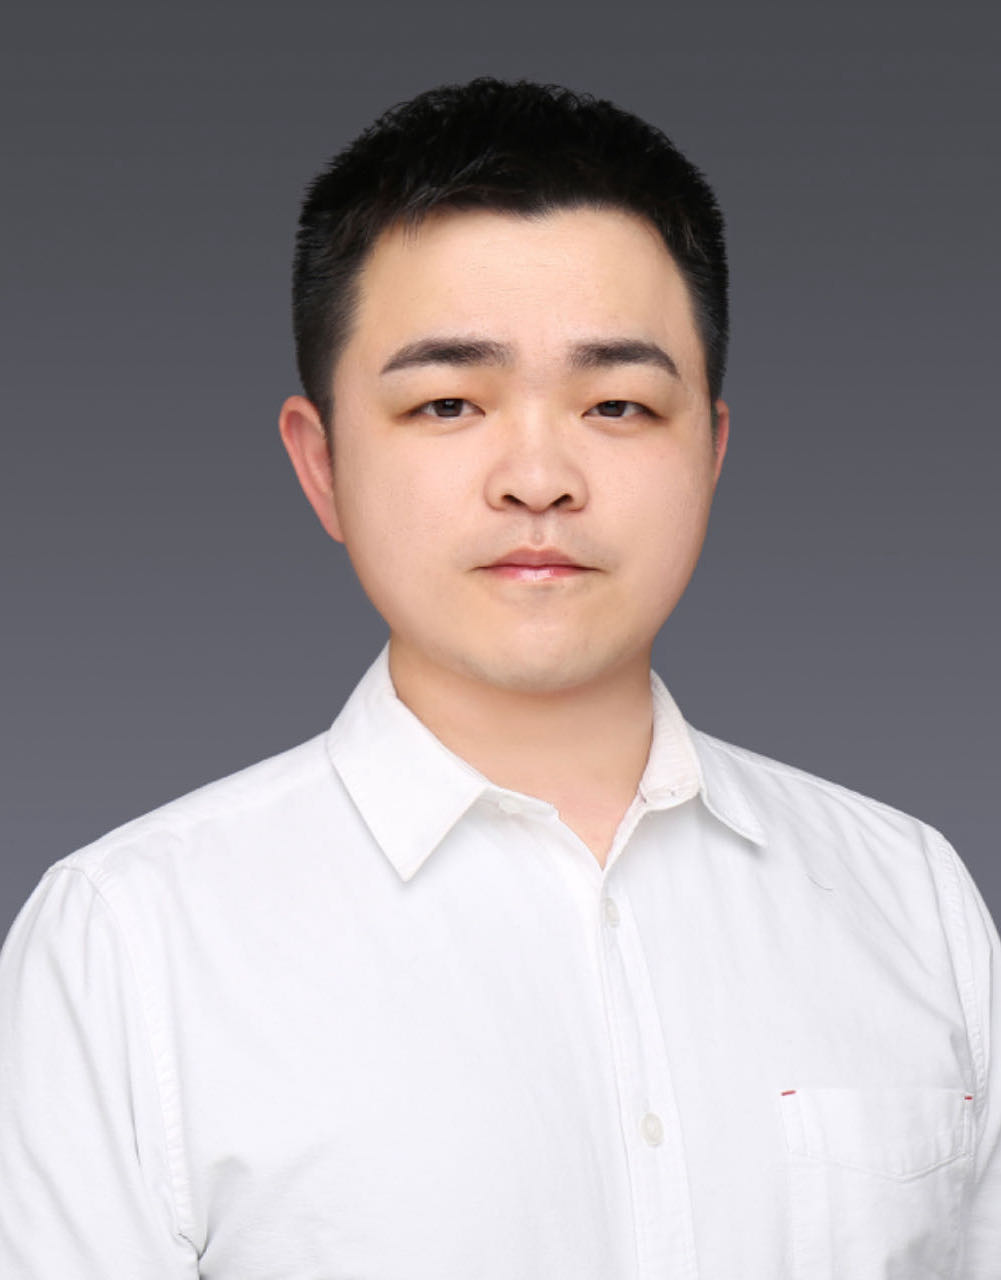
\includegraphics[width=1in,height=1.25in,clip,keepaspectratio]{figures/Xiaoyi_Gu.jpg}}]
   {Xiaoyi Gu} received the B.E. degree in Mechanical Engineering and Automation, M.E. degree and Ph.D. degree in Biomedical Engineering both from the National University of Singapore (NUS). Currently, he is with Joyo Medtech (Suzhou) Co., Ltd, Suzhou, China. His research interests include medical/surgical robotics and bioinpired robotics.
\end{IEEEbiography}


\end{document}
